\chapter{Diseño de clases} \label{cap:diseño_clases}

\section{Introducción}

En este capítulo se realizará una breve introducción sobre el diagrama de clases y posteriormente, un análisis de las clases que participan en el modelo de información del simulador SimAS 3.0. Para ello, se especificarán los atributos, métodos y las relaciones existentes entre las mismas, terminándose con un diagrama de clases general de todo el sistema.

El propósito de un diagrama de clases es el de representar los objetos fundamentales del sistema, es decir, los que percibe el usuario y con los que espera tratar para completar su tarea. Una clase define el ámbito de definición de un conjunto de objetos.

Cada clase se representa en un rectángulo con tres apartados:
\begin{itemize}
\item Nombre de la clase.
\item Atributos de la clase.
\item Operaciones de la clase.
\end{itemize}

En SimAS 3.0, el diseño de clases sigue el patrón Model-View-Controller (MVC), donde las clases del modelo representan la lógica de negocio y los datos de las gramáticas de contexto libre, mientras que las clases de la vista y controlador manejan la interfaz de usuario y la interacción con el usuario.


\section{Clases del sistema}

Según el análisis del sistema realizado hasta ahora, las clases \textbf{principales} que componen el sistema SimAS 3.0 son las siguientes:

\begin{itemize}
 \item \textbf{Bienvenida}: clase que gestiona la pantalla de bienvenida (extends Application).
 \item \textbf{MenuPrincipal}: clase que controla el menú principal de la aplicación (extends Application).
 \item \textbf{Editor}: clase principal del editor de gramáticas (extends VBox).
 \item \textbf{EditorWindow}: clase base para ventanas del editor.
 \item \textbf{SimulacionFinal}: clase principal del simulador (extends BorderPane).
 \item \textbf{AcercaDe}: clase que gestiona la ventana "Acerca de" (extends JDialog).
\end{itemize}

Las clases que representan el \textbf{modelo de datos} de las gramáticas de contexto libre son las siguientes:

\begin{itemize}
 \item \textbf{Gramatica}: clase principal que representa una gramática completa.
 \item \textbf{Produccion}: representa una regla de producción de la gramática.
 \item \textbf{Antecedente}: representa la parte izquierda de una producción.
 \item \textbf{Consecuente}: representa la parte derecha de una producción.
 \item \textbf{NoTerminal}: representa símbolos no terminales de la gramática.
 \item \textbf{Terminal}: representa símbolos terminales de la gramática.
 \item \textbf{Simbolo}: clase base para representar símbolos de la gramática.
 \item \textbf{TablaPredictiva}: implementa la tabla predictiva para análisis descendente.
 \item \textbf{TablaPredictivaPaso5}: extensión de TablaPredictiva con funciones de error.
 \item \textbf{FilaTablaPredictiva}: representa una fila de la tabla predictiva.
 \item \textbf{FuncionError}: representa funciones de tratamiento de errores.
\end{itemize}

Las clases del paquete \textbf{editor} que gestionan la interfaz de edición son:

\begin{itemize}
 \item \textbf{PanelCreacionGramatica}: panel principal para la creación de gramáticas (extends BorderPane).
 \item \textbf{PanelCreacionGramaticaPaso1} a \textbf{PanelCreacionGramaticaPaso4}: paneles del asistente de creación (extends VBox).
 \item \textbf{PanelProducciones}: panel para gestión de producciones (extends VBox).
 \item \textbf{PanelSimbolosNoTerminales}: panel para símbolos no terminales (extends VBox).
 \item \textbf{PanelSimbolosTerminales}: panel para símbolos terminales (extends VBox).
\end{itemize}

Las clases del paquete \textbf{simulador} que gestionan la simulación son:

\begin{itemize}
 \item \textbf{PanelSimuladorDesc}: panel principal del simulador descendente.
 \item \textbf{PanelNuevaSimDescPaso1} a \textbf{PanelNuevaSimDescPaso6}: paneles del asistente de simulación.
 \item \textbf{PanelSimulacion}: panel que muestra los resultados de la simulación (extends VBox).
 \item \textbf{PanelGramaticaOriginal}: panel para visualizar la gramática original (extends VBox).
 \item \textbf{NuevaFuncionError}: clase para gestión de funciones de error.
 \item \textbf{EditorCadenaEntradaController}: controlador para edición de cadenas de entrada.
\end{itemize}

Las clases que se encuentran en el paquete \textbf{utils} y proporcionan funcionalidades transversales son:

\begin{itemize}
 \item \textbf{ActualizableTextos}: interfaz para gestión de textos actualizables.
 \item \textbf{LanguageItem}: elementos de idioma para internacionalización.
 \item \textbf{LanguageListCell}: celda personalizada para lista de idiomas (extends ListCell).
 \item \textbf{SecondaryWindow}: ventanas secundarias de la aplicación (extends EditorWindow).
 \item \textbf{TabManager}: gestor de pestañas.
 \item \textbf{TabPaneMonitor}: monitor para control de pestañas.
\end{itemize}

A continuación se hará un análisis detallado de las clases más importantes del sistema.

\subsection{Clase Bienvenida}

Esta clase representa la pantalla de bienvenida de la aplicación SimAS 3.0, heredando de Application para ser el punto de entrada principal.

\begin{longtable}[H]{|>{\columncolor[rgb]{0.63,0.79,0.95}}m{6cm} | m{8.5cm} |}
 \caption{Clase Bienvenida}

\endfirsthead

\multicolumn{2}{c}
{{\tablename\ \thetable{} -- continúa de la página anterior}} \\
\endhead

\hline \multicolumn{2}{|r|}{{Continúa en la página siguiente}} \\ \hline
\endfoot

\hline
\endlastfoot

\hline
 \textbf{Nombre} & \textbf{Bienvenida}  \\ \hline
 
 \textbf{Descripción} & Representa la pantalla de bienvenida de la aplicación (extends Application).  \\ \hline
                       
 \textbf{Atributos} & \begin{enumerate}
 		\item \textbf{stage}: Stage principal de la aplicación.
 		\item \textbf{scene}: Scene que contiene la interfaz de bienvenida.
\end{enumerate} \\ \hline
 
 \textbf{Métodos} & \begin{enumerate}
 		\item \textbf{start(Stage)}: método principal que inicializa la aplicación.
 		\item \textbf{main(String[])}: punto de entrada de la aplicación.
\end{enumerate}
                                 
 \label{tabla98}

\end{longtable}

\subsection{Clase MenuPrincipal}

Esta clase gestiona el menú principal de la aplicación, proporcionando acceso a las diferentes funcionalidades.

\begin{longtable}[H]{|>{\columncolor[rgb]{0.63,0.79,0.95}}m{6cm} | m{8.5cm} |}
 \caption{Clase MenuPrincipal}

\endfirsthead

\multicolumn{2}{c}
{{\tablename\ \thetable{} -- continúa de la página anterior}} \\
\endhead

\hline \multicolumn{2}{|r|}{{Continúa en la página siguiente}} \\ \hline
\endfoot

\hline
\endlastfoot

\hline
 \textbf{Nombre} & \textbf{MenuPrincipal}  \\ \hline
 
 \textbf{Descripción} & Gestiona el menú principal de la aplicación (extends Application).  \\ \hline
                       
 \textbf{Atributos} & \begin{enumerate}
 		\item \textbf{stage}: Stage principal de la aplicación.
 		\item \textbf{scene}: Scene que contiene el menú principal.
\end{enumerate} \\ \hline
 
 \textbf{Métodos} & \begin{enumerate}
 		\item \textbf{start(Stage)}: inicializa el menú principal.
 		\item \textbf{abrirEditor()}: abre la ventana del editor.
 		\item \textbf{abrirSimulador()}: abre la ventana del simulador.
 		\item \textbf{abrirAyuda()}: abre el sistema de ayuda.
\end{enumerate}
                                 
 \label{tabla99}

\end{longtable}

\subsection{Clase Gramatica}

Esta clase representa el núcleo del modelo de datos de SimAS 3.0, conteniendo toda la información de una gramática de contexto libre. Es la clase más compleja del sistema y está diseñada para trabajar con JavaFX, utilizando propiedades observables para el binding con la interfaz de usuario.

\begin{longtable}[H]{|>{\columncolor[rgb]{0.63,0.79,0.95}}m{6cm} | m{8.5cm} |}
 \caption{Clase Gramatica}

\endfirsthead

\multicolumn{2}{c}
{{\tablename\ \thetable{} -- continúa de la página anterior}} \\
\endhead

\hline \multicolumn{2}{|r|}{{Continúa en la página siguiente}} \\ \hline
\endfoot

\hline
\endlastfoot

\hline
 \textbf{Nombre} & \textbf{Gramatica}  \\ \hline
 
 \textbf{Descripción} & Representa una gramática de contexto libre completa con todas sus propiedades y funcionalidades.  \\ \hline
                       
 \textbf{Atributos} & \begin{enumerate}
 		\item \textbf{nombre}: StringProperty que representa el nombre de la gramática.
 		\item \textbf{descripcion}: StringProperty que contiene la descripción de la gramática.
 		\item \textbf{simbInicial}: StringProperty que representa el símbolo inicial.
 		\item \textbf{archivoFuente}: StringProperty que contiene la ruta del archivo fuente.
 		\item \textbf{estado}: IntegerProperty que indica el estado actual de la gramática.
 		\item \textbf{terminales}: ObservableList\<Terminal\> que contiene los símbolos terminales.
 		\item \textbf{noTerminales}: ObservableList\<NoTerminal\> que contiene los símbolos no terminales.
 		\item \textbf{pr}: ObservableList\<Produccion\> que contiene las producciones.
 		\item \textbf{tpredictiva}: TablaPredictiva que implementa la tabla predictiva.
\end{enumerate} \\ \hline
 
 \textbf{Métodos} & \begin{enumerate}
 		\item \textbf{getNombre()}: obtiene el nombre de la gramática.
 		\item \textbf{setNombre(String)}: establece el nombre de la gramática.
 		\item \textbf{getDescripcion()}: obtiene la descripción de la gramática.
 		\item \textbf{setDescripcion(String)}: establece la descripción de la gramática.
 		\item \textbf{getSimbInicial()}: obtiene el símbolo inicial.
 		\item \textbf{setSimbInicial(String)}: establece el símbolo inicial.
 		\item \textbf{getTerminales()}: obtiene la lista de terminales.
 		\item \textbf{getNoTerminales()}: obtiene la lista de no terminales.
 		\item \textbf{getProducciones()}: obtiene la lista de producciones.
 		\item \textbf{getTablaPredictiva()}: obtiene la tabla predictiva.
 		\item \textbf{generarTablaPredictiva()}: genera la tabla predictiva.
 		\item \textbf{validarGramatica()}: valida la gramática.
\end{enumerate}
                                 
 \label{tabla100}

\end{longtable}

\subsection{Clase Simbolo}

Esta clase representa la clase base para todos los símbolos de la gramática, tanto terminales como no terminales.

\begin{longtable}[H]{|>{\columncolor[rgb]{0.63,0.79,0.95}}m{6cm} | m{8.5cm} |}
 \caption{Clase Simbolo}

\endfirsthead

\multicolumn{2}{c}
{{\tablename\ \thetable{} -- continúa de la página anterior}} \\
\endhead

\hline \multicolumn{2}{|r|}{{Continúa en la página siguiente}} \\ \hline
\endfoot

\hline
\endlastfoot

\hline
 \textbf{Nombre} & \textbf{Simbolo}  \\ \hline
 
 \textbf{Descripción} & Clase base abstracta que representa un símbolo de la gramática.  \\ \hline
                       
 \textbf{Atributos} & \begin{enumerate}
 		\item \textbf{nombre}: StringProperty que representa el nombre del símbolo.
 		\item \textbf{valor}: StringProperty que contiene el valor del símbolo.
\end{enumerate} \\ \hline
 
 \textbf{Métodos} & \begin{enumerate}
 		\item \textbf{getNombre()}: obtiene el nombre del símbolo.
 		\item \textbf{setNombre(String)}: establece el nombre del símbolo.
 		\item \textbf{getValor()}: obtiene el valor del símbolo.
 		\item \textbf{setValor(String)}: establece el valor del símbolo.
 		\item \textbf{nombreProperty()}: obtiene la propiedad observable del nombre.
 		\item \textbf{valorProperty()}: obtiene la propiedad observable del valor.
\end{enumerate}
                                 
 \label{tabla101}

\end{longtable}

\subsection{Clase Terminal}

Esta clase representa los símbolos terminales de la gramática, heredando de la clase Simbolo.

\begin{longtable}[H]{|>{\columncolor[rgb]{0.63,0.79,0.95}}m{6cm} | m{8.5cm} |}
 \caption{Clase Terminal}

\endfirsthead

\multicolumn{2}{c}
{{\tablename\ \thetable{} -- continúa de la página anterior}} \\
\endhead

\hline \multicolumn{2}{|r|}{{Continúa en la página siguiente}} \\ \hline
\endfoot

\hline
\endlastfoot

\hline
 \textbf{Nombre} & \textbf{Terminal}  \\ \hline
 
 \textbf{Descripción} & Representa un símbolo terminal de la gramática (extends Simbolo).  \\ \hline
                       
 \textbf{Atributos} & Hereda todos los atributos de la clase Simbolo.  \\ \hline
 
 \textbf{Métodos} & \begin{enumerate}
 		\item \textbf{Terminal(String)}: constructor que inicializa el terminal con un nombre.
 		\item \textbf{Terminal(String, String)}: constructor que inicializa el terminal con nombre y valor.
 		\item Hereda todos los métodos de la clase Simbolo.
\end{enumerate}
                                 
 \label{tabla102}

\end{longtable}

\subsection{Clase NoTerminal}

Esta clase representa los símbolos no terminales de la gramática, heredando de la clase Simbolo.

\begin{longtable}[H]{|>{\columncolor[rgb]{0.63,0.79,0.95}}m{6cm} | m{8.5cm} |}
 \caption{Clase NoTerminal}

\endfirsthead

\multicolumn{2}{c}
{{\tablename\ \thetable{} -- continúa de la página anterior}} \\
\endhead

\hline \multicolumn{2}{|r|}{{Continúa en la página siguiente}} \\ \hline
\endfoot

\hline
\endlastfoot

\hline
 \textbf{Nombre} & \textbf{NoTerminal}  \\ \hline
 
 \textbf{Descripción} & Representa un símbolo no terminal de la gramática (extends Simbolo).  \\ \hline
                       
 \textbf{Atributos} & Hereda todos los atributos de la clase Simbolo.  \\ \hline
 
 \textbf{Métodos} & \begin{enumerate}
 		\item \textbf{NoTerminal(String)}: constructor que inicializa el no terminal con un nombre.
 		\item \textbf{NoTerminal(String, String)}: constructor que inicializa el no terminal con nombre y valor.
 		\item Hereda todos los métodos de la clase Simbolo.
\end{enumerate}
                                 
 \label{tabla103}

\end{longtable}

\subsection{Clase Produccion}

Esta clase representa una regla de producción de la gramática, conteniendo un antecedente y un consecuente.

\begin{longtable}[H]{|>{\columncolor[rgb]{0.63,0.79,0.95}}m{6cm} | m{8.5cm} |}
 \caption{Clase Produccion}

\endfirsthead

\multicolumn{2}{c}
{{\tablename\ \thetable{} -- continúa de la página anterior}} \\
\endhead

\hline \multicolumn{2}{|r|}{{Continúa en la página siguiente}} \\ \hline
\endfoot

\hline
\endlastfoot

\hline
 \textbf{Nombre} & \textbf{Produccion}  \\ \hline
 
 \textbf{Descripción} & Representa una regla de producción de la gramática con antecedente y consecuente.  \\ \hline
                       
 \textbf{Atributos} & \begin{enumerate}
 		\item \textbf{antec}: Antecedente que representa la parte izquierda de la producción.
 		\item \textbf{consec}: ObservableList\<Simbolo\> que representa la parte derecha de la producción.
 		\item \textbf{numero}: int que representa el número de la producción.
\end{enumerate} \\ \hline
 
 \textbf{Métodos} & \begin{enumerate}
 		\item \textbf{getAntec()}: obtiene el antecedente de la producción.
 		\item \textbf{setAntec(Antecedente)}: establece el antecedente de la producción.
 		\item \textbf{getConsec()}: obtiene el consecuente de la producción.
 		\item \textbf{setConsec(ObservableList\<Simbolo\>)}: establece el consecuente de la producción.
 		\item \textbf{getNumero()}: obtiene el número de la producción.
 		\item \textbf{setNumero(int)}: establece el número de la producción.
\end{enumerate}
                                 
 \label{tabla104}

\end{longtable}

\subsection{Clase Antecedente}

Esta clase representa la parte izquierda de una producción, conteniendo un símbolo no terminal.

\begin{longtable}[H]{|>{\columncolor[rgb]{0.63,0.79,0.95}}m{6cm} | m{8.5cm} |}
 \caption{Clase Antecedente}

\endfirsthead

\multicolumn{2}{c}
{{\tablename\ \thetable{} -- continúa de la página anterior}} \\
\endhead

\hline \multicolumn{2}{|r|}{{Continúa en la página siguiente}} \\ \hline
\endfoot

\hline
\endlastfoot

\hline
 \textbf{Nombre} & \textbf{Antecedente}  \\ \hline
 
 \textbf{Descripción} & Representa la parte izquierda de una producción (símbolo no terminal).  \\ \hline
                       
 \textbf{Atributos} & \begin{enumerate}
 		\item \textbf{noTerminal}: NoTerminal que representa el símbolo no terminal del antecedente.
\end{enumerate} \\ \hline
 
 \textbf{Métodos} & \begin{enumerate}
 		\item \textbf{getNoTerminal()}: obtiene el símbolo no terminal del antecedente.
 		\item \textbf{setNoTerminal(NoTerminal)}: establece el símbolo no terminal del antecedente.
\end{enumerate}
                                 
 \label{tabla105}

\end{longtable}

\subsection{Clase Consecuente}

Esta clase representa la parte derecha de una producción, conteniendo una lista de símbolos.

\begin{longtable}[H]{|>{\columncolor[rgb]{0.63,0.79,0.95}}m{6cm} | m{8.5cm} |}
 \caption{Clase Consecuente}

\endfirsthead

\multicolumn{2}{c}
{{\tablename\ \thetable{} -- continúa de la página anterior}} \\
\endhead

\hline \multicolumn{2}{|r|}{{Continúa en la página siguiente}} \\ \hline
\endfoot

\hline
\endlastfoot

\hline
 \textbf{Nombre} & \textbf{Consecuente}  \\ \hline
 
 \textbf{Descripción} & Representa la parte derecha de una producción (lista de símbolos).  \\ \hline
                       
 \textbf{Atributos} & \begin{enumerate}
 		\item \textbf{simbolos}: ObservableList\<Simbolo\> que contiene los símbolos del consecuente.
\end{enumerate} \\ \hline
 
 \textbf{Métodos} & \begin{enumerate}
 		\item \textbf{getSimbolos()}: obtiene la lista de símbolos del consecuente.
 		\item \textbf{setSimbolos(ObservableList\<Simbolo\>)}: establece la lista de símbolos del consecuente.
 		\item \textbf{addSimbolo(Simbolo)}: añade un símbolo al consecuente.
 		\item \textbf{removeSimbolo(Simbolo)}: elimina un símbolo del consecuente.
\end{enumerate}
                                 
 \label{tabla106}

\end{longtable}

\subsection{Clase TablaPredictiva}

Esta clase representa la tabla predictiva utilizada en el análisis sintáctico descendente predictivo, implementando la estructura de datos necesaria para el algoritmo de parsing.

\begin{longtable}[H]{|>{\columncolor[rgb]{0.63,0.79,0.95}}m{6cm} | m{8.5cm} |}
 \caption{Clase TablaPredictiva}

\endfirsthead

\multicolumn{2}{c}
{{\tablename\ \thetable{} -- continúa de la página anterior}} \\
\endhead

\hline \multicolumn{2}{|r|}{{Continúa en la página siguiente}} \\ \hline
\endfoot

\hline
\endlastfoot

\hline
 \textbf{Nombre} & \textbf{TablaPredictiva}  \\ \hline
 
 \textbf{Descripción} & Representa la tabla predictiva para análisis sintáctico descendente predictivo.  \\ \hline
                       
 \textbf{Atributos} & \begin{enumerate}
 		\item \textbf{tablaPredictiva}: TableView\<FilaTablaPredictiva\> que contiene la interfaz de la tabla.
 		\item \textbf{gramatica}: Gramatica asociada a la tabla predictiva.
 		\item \textbf{indiceColumnas}: Map\<String, Integer\> que mapea nombres de columnas a índices.
 		\item \textbf{funcionesError}: List\<FuncionError\> que contiene las funciones de manejo de errores.
 		\item \textbf{bundle}: ResourceBundle para internacionalización.
\end{enumerate} \\ \hline
 
 \textbf{Métodos} & \begin{enumerate}
 		\item \textbf{construir(Gramatica)}: construye la tabla predictiva a partir de una gramática.
 		\item \textbf{cargarDatos()}: carga los datos de la gramática en la tabla.
 		\item \textbf{crearFunError(FuncionError)}: añade una función de error a la tabla.
 		\item \textbf{getFuncionesError()}: obtiene la lista de funciones de error.
 		\item \textbf{setFuncionesError(List\<FuncionError\>)}: establece las funciones de error.
 		\item \textbf{getTablaPredictiva()}: obtiene la tabla de interfaz de usuario.
 		\item \textbf{getFilas()}: obtiene las filas de la tabla.
 		\item \textbf{getColumnas()}: obtiene el número de columnas.
\end{enumerate}
                                 
 \label{tabla107}

\end{longtable}

\subsection{Clase TablaPredictivaPaso5}

Esta clase extiende TablaPredictiva para proporcionar funcionalidades específicas del paso 5 del simulador, incluyendo manejo de funciones de error y terminales.

\begin{longtable}[H]{|>{\columncolor[rgb]{0.63,0.79,0.95}}m{6cm} | m{8.5cm} |}
 \caption{Clase TablaPredictivaPaso5}

\endfirsthead

\multicolumn{2}{c}
{{\tablename\ \thetable{} -- continúa de la página anterior}} \\
\endhead

\hline \multicolumn{2}{|r|}{{Continúa en la página siguiente}} \\ \hline
\endfoot

\hline
\endlastfoot

\hline
 \textbf{Nombre} & \textbf{TablaPredictivaPaso5}  \\ \hline
 
 \textbf{Descripción} & Extensión de TablaPredictiva para el paso 5 del simulador (extends TablaPredictiva).  \\ \hline
                       
 \textbf{Atributos} & \begin{enumerate}
 		\item \textbf{panelPaso5}: PanelNuevaSimDescPaso5 que contiene el panel asociado.
 		\item \textbf{funcionesError}: List\<FuncionError\> específica para el paso 5.
 		\item \textbf{columnsCreated}: boolean que indica si las columnas han sido creadas.
\end{enumerate} \\ \hline
 
 \textbf{Métodos} & \begin{enumerate}
 		\item \textbf{setPanelPaso5(PanelNuevaSimDescPaso5)}: establece el panel asociado.
 		\item \textbf{apareceSoloPrimeraPos(Terminal)}: verifica si un terminal aparece solo en primera posición.
 		\item \textbf{rellenarProduccionesEpsilon()}: rellena las producciones épsilon en la tabla.
 		\item \textbf{construir(Gramatica)}: construye la tabla con funcionalidades específicas del paso 5.
 		\item \textbf{crearColumnas(Gramatica)}: crea las columnas de la tabla.
 		\item \textbf{cargarDatos()}: carga datos incluyendo terminales.
 		\item \textbf{configurarColumnas()}: configura el estilo de las columnas.
 		\item \textbf{configurarSeleccion()}: configura la selección de celdas.
 		\item \textbf{configurarManejadorClics()}: configura el manejo de clics en celdas.
\end{enumerate}
                                 
 \label{tabla108}

\end{longtable}

\subsection{Clase FilaTablaPredictiva}

Esta clase representa una fila individual de la tabla predictiva, asociando un símbolo con sus valores correspondientes en cada columna.

\begin{longtable}[H]{|>{\columncolor[rgb]{0.63,0.79,0.95}}m{6cm} | m{8.5cm} |}
 \caption{Clase FilaTablaPredictiva}

\endfirsthead

\multicolumn{2}{c}
{{\tablename\ \thetable{} -- continúa de la página anterior}} \\
\endhead

\hline \multicolumn{2}{|r|}{{Continúa en la página siguiente}} \\ \hline
\endfoot

\hline
\endlastfoot

\hline
 \textbf{Nombre} & \textbf{FilaTablaPredictiva}  \\ \hline
 
 \textbf{Descripción} & Representa una fila de la tabla predictiva con un símbolo y sus valores por columna.  \\ \hline
                       
 \textbf{Atributos} & \begin{enumerate}
 		\item \textbf{simbolo}: StringProperty que representa el símbolo de la fila.
 		\item \textbf{prediccion}: StringProperty que contiene la predicción de la fila.
 		\item \textbf{valoresColumnas}: Map\<String, StringProperty\> que mapea nombres de columnas a valores.
 		\item \textbf{esTerminal}: BooleanProperty que indica si la fila representa un terminal.
 		\item \textbf{celdasConProduccion}: Map\<String, Boolean\> que indica qué celdas contienen producciones.
\end{enumerate} \\ \hline
 
 \textbf{Métodos} & \begin{enumerate}
 		\item \textbf{getSimbolo()}: obtiene el símbolo de la fila.
 		\item \textbf{setSimbolo(String)}: establece el símbolo de la fila.
 		\item \textbf{getPrediccion()}: obtiene la predicción de la fila.
 		\item \textbf{setPrediccion(String)}: establece la predicción de la fila.
 		\item \textbf{setValor(String, String)}: establece el valor de una columna específica.
 		\item \textbf{getValor(String)}: obtiene el valor de una columna específica.
 		\item \textbf{getEsTerminal()}: indica si la fila representa un terminal.
 		\item \textbf{setEsTerminal(boolean)}: establece si la fila representa un terminal.
 		\item \textbf{setProduccionEnCelda(String, boolean)}: marca si una celda contiene una producción.
 		\item \textbf{tieneProduccionEnCelda(String)}: verifica si una celda contiene una producción.
\end{enumerate}
                                 
 \label{tabla109}

\end{longtable}

\subsection{Clase FuncionError}

Esta clase representa una función de manejo de errores en la tabla predictiva, definiendo las acciones a realizar cuando se produce un error durante el análisis sintáctico.

\begin{longtable}[H]{|>{\columncolor[rgb]{0.63,0.79,0.95}}m{6cm} | m{8.5cm} |}
 \caption{Clase FuncionError}

\endfirsthead

\multicolumn{2}{c}
{{\tablename\ \thetable{} -- continúa de la página anterior}} \\
\endhead

\hline \multicolumn{2}{|r|}{{Continúa en la página siguiente}} \\ \hline
\endfoot

\hline
\endlastfoot

\hline
 \textbf{Nombre} & \textbf{FuncionError}  \\ \hline
 
 \textbf{Descripción} & Representa una función de manejo de errores en la tabla predictiva.  \\ \hline
                       
 \textbf{Atributos} & \begin{enumerate}
 		\item \textbf{identificador}: int que identifica únicamente la función de error.
 		\item \textbf{accion}: int que define el tipo de acción a realizar.
 		\item \textbf{mensaje}: String que contiene el mensaje descriptivo de la función.
 		\item \textbf{simbolo}: Terminal asociado a la función de error.
\end{enumerate} \\ \hline
 
 \textbf{Métodos} & \begin{enumerate}
 		\item \textbf{getIdentificador()}: obtiene el identificador de la función.
 		\item \textbf{setIdentificador(int)}: establece el identificador de la función.
 		\item \textbf{getAccion()}: obtiene el tipo de acción.
 		\item \textbf{setAccion(int)}: establece el tipo de acción.
 		\item \textbf{getMensaje()}: obtiene el mensaje de la función.
 		\item \textbf{setMensaje(String)}: establece el mensaje de la función.
 		\item \textbf{getSimbolo()}: obtiene el símbolo asociado.
 		\item \textbf{setSimbolo(Terminal)}: establece el símbolo asociado.
 		\item \textbf{getNombreAccion()}: obtiene el nombre descriptivo de la acción.
 		\item \textbf{equals(Object)}: compara dos funciones de error.
 		\item \textbf{hashCode()}: calcula el hash de la función.
 		\item \textbf{toString()}: representa la función como cadena.
\end{enumerate}
                                 
 \label{tabla110}

\end{longtable}

\subsection{Clase Editor}

Esta clase representa el editor principal de gramáticas de contexto libre, proporcionando una interfaz completa para crear, editar, validar y gestionar gramáticas.

\begin{longtable}[H]{|>{\columncolor[rgb]{0.63,0.79,0.95}}m{6cm} | m{8.5cm} |}
 \caption{Clase Editor}

\endfirsthead

\multicolumn{2}{c}
{{\tablename\ \thetable{} -- continúa de la página anterior}} \\
\endhead

\hline \multicolumn{2}{|r|}{{Continúa en la página siguiente}} \\ \hline
\endfoot

\hline
\endlastfoot

\hline
 \textbf{Nombre} & \textbf{Editor}  \\ \hline
 
 \textbf{Descripción} & Editor principal de gramáticas de contexto libre (extends VBox, implements ActualizableTextos).  \\ \hline
                       
 \textbf{Atributos} & \begin{enumerate}
 		\item \textbf{gramatica}: Gramatica que representa la gramática actual del editor.
 		\item \textbf{tabPane}: TabPane para gestión de pestañas.
 		\item \textbf{menuPane}: MenuPrincipal para navegación.
 		\item \textbf{bundle}: ResourceBundle para internacionalización.
 		\item \textbf{editorId}: String que identifica únicamente este editor.
 		\item \textbf{listenerConfigured}: boolean que indica si los listeners están configurados.
 		\item \textbf{rootPane}: BorderPane que contiene la interfaz principal.
 		\item \textbf{listNoTerminales}: ListView\<String\> para mostrar no terminales.
 		\item \textbf{listTerminales}: ListView\<String\> para mostrar terminales.
 		\item \textbf{listProducciones}: ListView\<String\> para mostrar producciones.
\end{enumerate} \\ \hline
 
 \textbf{Métodos} & \begin{enumerate}
 		\item \textbf{getGramatica()}: obtiene la gramática actual.
 		\item \textbf{setGramatica(Gramatica)}: establece la gramática.
 		\item \textbf{getEditorId()}: obtiene el ID único del editor.
 		\item \textbf{cargarGramatica()}: carga una gramática desde archivo.
 		\item \textbf{grabarGramatica()}: guarda la gramática en archivo.
 		\item \textbf{validarGramatica(Gramatica)}: valida la gramática.
 		\item \textbf{actualizarVisualizacion()}: actualiza la interfaz con los datos de la gramática.
 		\item \textbf{generarInformePDF()}: genera un informe PDF de la gramática.
 		\item \textbf{actualizarTextos(ResourceBundle)}: actualiza los textos de la interfaz.
 		\item \textbf{configurarRelacionesPadreHijo()}: configura las relaciones entre pestañas.
\end{enumerate}
                                 
 \label{tabla111}

\end{longtable}

\subsection{Clase EditorWindow}

Esta clase representa una ventana de editor que puede contener múltiples pestañas con editores y simuladores, proporcionando funcionalidades avanzadas de gestión de ventanas.

\begin{longtable}[H]{|>{\columncolor[rgb]{0.63,0.79,0.95}}m{6cm} | m{8.5cm} |}
 \caption{Clase EditorWindow}

\endfirsthead

\multicolumn{2}{c}
{{\tablename\ \thetable{} -- continúa de la página anterior}} \\
\endhead

\hline \multicolumn{2}{|r|}{{Continúa en la página siguiente}} \\ \hline
\endfoot

\hline
\endlastfoot

\hline
 \textbf{Nombre} & \textbf{EditorWindow}  \\ \hline
 
 \textbf{Descripción} & Ventana de editor que gestiona múltiples pestañas con editores y simuladores.  \\ \hline
                       
 \textbf{Atributos} & \begin{enumerate}
 		\item \textbf{stage}: Stage que representa la ventana principal.
 		\item \textbf{tabPane}: TabPane que gestiona las pestañas de la ventana.
 		\item \textbf{bundle}: ResourceBundle para internacionalización.
\end{enumerate} \\ \hline
 
 \textbf{Métodos} & \begin{enumerate}
 		\item \textbf{show()}: muestra la ventana.
 		\item \textbf{addTab(Tab)}: añade una pestaña a la ventana.
 		\item \textbf{addEditor(Editor)}: añade un editor a la ventana.
 		\item \textbf{getTabPane()}: obtiene el TabPane de la ventana.
 		\item \textbf{moveGroupToWindow(TabPane, String, Tab)}: mueve un grupo de pestañas a esta ventana.
 		\item \textbf{configurarAtajosTeclado(Scene)}: configura los atajos de teclado.
 		\item \textbf{abrirEditorEnEditorWindow()}: abre un nuevo editor en esta ventana.
 		\item \textbf{abrirSimuladorEnEditorWindow()}: abre un simulador en esta ventana.
\end{enumerate}
                                 
\label{tabla112}

\end{longtable}

\subsection{Clase PanelCreacionGramatica}

Esta clase representa el asistente principal para la creación y edición de gramáticas, coordinando los diferentes pasos del proceso.

\begin{longtable}[H]{|>{\columncolor[rgb]{0.63,0.79,0.95}}m{6cm} | m{8.5cm} |}
 \caption{Clase PanelCreacionGramatica}

\endfirsthead

\multicolumn{2}{c}
{{\tablename\ \thetable{} -- continúa de la página anterior}} \\
\endhead

\hline \multicolumn{2}{|r|}{{Continúa en la página siguiente}} \\ \hline
\endfoot

\hline
\endlastfoot

\hline
 \textbf{Nombre} & \textbf{PanelCreacionGramatica}  \\ \hline
 
 \textbf{Descripción} & Asistente principal para creación y edición de gramáticas (extends BorderPane, implements ActualizableTextos).  \\ \hline
                       
 \textbf{Atributos} & \begin{enumerate}
 		\item \textbf{tabPane}: TabPane para gestión de pestañas.
 		\item \textbf{paso1}: PanelCreacionGramaticaPaso1 para el primer paso.
 		\item \textbf{paso2}: PanelCreacionGramaticaPaso2 para el segundo paso.
 		\item \textbf{paso3}: PanelCreacionGramaticaPaso3 para el tercer paso.
 		\item \textbf{paso4}: PanelCreacionGramaticaPaso4 para el cuarto paso.
 		\item \textbf{panelPadre}: Editor que contiene este asistente.
 		\item \textbf{menuPane}: MenuPrincipal para navegación.
 		\item \textbf{gramaticaTemporal}: Gramatica temporal para la edición.
 		\item \textbf{bundle}: ResourceBundle para internacionalización.
 		\item \textbf{creacionId}: String que identifica únicamente esta creación.
\end{enumerate} \\ \hline
 
 \textbf{Métodos} & \begin{enumerate}
 		\item \textbf{getGramatica()}: obtiene la gramática temporal.
 		\item \textbf{setGramatica(Gramatica)}: establece la gramática temporal.
 		\item \textbf{cambiarPaso(int)}: cambia al paso especificado del asistente.
 		\item \textbf{getCreacionId()}: obtiene el ID único de la creación.
 		\item \textbf{cancelarEdicion()}: cancela la edición actual.
 		\item \textbf{mostrarAlerta(String, String)}: muestra una alerta al usuario.
 		\item \textbf{actualizarTextos(ResourceBundle)}: actualiza los textos de la interfaz.
 		\item \textbf{configurarRelacionesPadreHijo()}: configura las relaciones entre pestañas.
\end{enumerate}
                                 
 \label{tabla113}

\end{longtable}

\subsection{Clase PanelCreacionGramaticaPaso1}

Esta clase representa el primer paso del asistente de creación de gramáticas, donde se introducen el nombre y la descripción.

\begin{longtable}[H]{|>{\columncolor[rgb]{0.63,0.79,0.95}}m{6cm} | m{8.5cm} |}
 \caption{Clase PanelCreacionGramaticaPaso1}

\endfirsthead

\multicolumn{2}{c}
{{\tablename\ \thetable{} -- continúa de la página anterior}} \\
\endhead

\hline \multicolumn{2}{|r|}{{Continúa en la página siguiente}} \\ \hline
\endfoot

\hline
\endlastfoot

\hline
 \textbf{Nombre} & \textbf{PanelCreacionGramaticaPaso1}  \\ \hline
 
 \textbf{Descripción} & Primer paso del asistente para introducir nombre y descripción (extends VBox, implements ActualizableTextos).  \\ \hline
                       
 \textbf{Atributos} & \begin{enumerate}
 		\item \textbf{txtNombre}: TextField para introducir el nombre de la gramática.
 		\item \textbf{txtDescripcion}: TextArea para introducir la descripción.
 		\item \textbf{btnSiguiente}: Button para avanzar al siguiente paso.
 		\item \textbf{btnAnterior}: Button para retroceder al paso anterior.
 		\item \textbf{btnCancelar}: Button para cancelar la creación.
 		\item \textbf{btnUltimo}: Button para ir al último paso.
 		\item \textbf{btnPrimero}: Button para ir al primer paso.
 		\item \textbf{lblNombreError}: Label para mostrar errores del nombre.
 		\item \textbf{lblDescripcionError}: Label para mostrar errores de la descripción.
 		\item \textbf{panelPadre}: PanelCreacionGramatica que contiene este paso.
 		\item \textbf{bundle}: ResourceBundle para internacionalización.
\end{enumerate} \\ \hline
 
 \textbf{Métodos} & \begin{enumerate}
 		\item \textbf{setNombre(String)}: establece el nombre de la gramática.
 		\item \textbf{setDescripcion(String)}: establece la descripción de la gramática.
 		\item \textbf{configurarValidaciones()}: configura las validaciones de los campos.
 		\item \textbf{datosValidos()}: verifica si los datos introducidos son válidos.
 		\item \textbf{hayDatosSinGuardar()}: verifica si hay datos sin guardar.
 		\item \textbf{determinarPasoUltimo()}: determina el último paso al que se puede ir.
 		\item \textbf{actualizarTextos(ResourceBundle)}: actualiza los textos de la interfaz.
\end{enumerate}
                                 
 \label{tabla114}

\end{longtable}

\subsection{Clase PanelProducciones}

Esta clase representa un panel especializado para la gestión de producciones de la gramática, permitiendo crear, modificar y eliminar reglas de producción.

\begin{longtable}[H]{|>{\columncolor[rgb]{0.63,0.79,0.95}}m{6cm} | m{8.5cm} |}
 \caption{Clase PanelProducciones}

\endfirsthead

\multicolumn{2}{c}
{{\tablename\ \thetable{} -- continúa de la página anterior}} \\
\endhead

\hline \multicolumn{2}{|r|}{{Continúa en la página siguiente}} \\ \hline
\endfoot

\hline
\endlastfoot

\hline
 \textbf{Nombre} & \textbf{PanelProducciones}  \\ \hline
 
 \textbf{Descripción} & Panel especializado para gestión de producciones de la gramática (extends VBox, implements ActualizableTextos).  \\ \hline
                       
 \textbf{Atributos} & \begin{enumerate}
 		\item \textbf{comboBoxAntecedente}: ComboBox\<NoTerminal\> para seleccionar el antecedente.
 		\item \textbf{txtConsecuente}: TextField para mostrar el consecuente.
 		\item \textbf{listProducciones}: ListView\<Produccion\> para mostrar las producciones.
 		\item \textbf{listTerminales}: ListView\<Simbolo\> para mostrar terminales disponibles.
 		\item \textbf{listNoTerminales}: ListView\<Simbolo\> para mostrar no terminales disponibles.
 		\item \textbf{btnInsertar}: Button para insertar nuevas producciones.
 		\item \textbf{btnModificar}: Button para modificar producciones existentes.
 		\item \textbf{btnEliminar}: Button para eliminar producciones.
 		\item \textbf{btnEpsilon}: Button para añadir símbolo épsilon.
 		\item \textbf{panelPadre}: PanelCreacionGramaticaPaso3 que contiene este panel.
 		\item \textbf{producciones}: ObservableList\<Produccion\> con las producciones.
 		\item \textbf{produccionSeleccionada}: Produccion actualmente seleccionada.
\end{enumerate} \\ \hline
 
 \textbf{Métodos} & \begin{enumerate}
 		\item \textbf{cargarProduccionParaModificar(Produccion)}: carga una producción para modificación.
 		\item \textbf{agregarSimboloAlConsecuente(Simbolo)}: añade un símbolo al consecuente.
 		\item \textbf{cerrarPestanaActual()}: cierra la pestaña actual.
 		\item \textbf{mostrarAlerta(String)}: muestra una alerta al usuario.
 		\item \textbf{actualizarTextos(ResourceBundle)}: actualiza los textos de la interfaz.
\end{enumerate}
                                 
 \label{tabla115}

\end{longtable}

\subsection{Clase PanelSimbolosNoTerminales}

Esta clase representa un panel especializado para la gestión de símbolos no terminales de la gramática.

\begin{longtable}[H]{|>{\columncolor[rgb]{0.63,0.79,0.95}}m{6cm} | m{8.5cm} |}
 \caption{Clase PanelSimbolosNoTerminales}

\endfirsthead

\multicolumn{2}{c}
{{\tablename\ \thetable{} -- continúa de la página anterior}} \\
\endhead

\hline \multicolumn{2}{|r|}{{Continúa en la página siguiente}} \\ \hline
\endfoot

\hline
\endlastfoot

\hline
 \textbf{Nombre} & \textbf{PanelSimbolosNoTerminales}  \\ \hline
 
 \textbf{Descripción} & Panel especializado para gestión de símbolos no terminales (extends VBox, implements ActualizableTextos).  \\ \hline
                       
 \textbf{Atributos} & \begin{enumerate}
 		\item \textbf{symbolButtonsPane}: FlowPane que contiene botones de símbolos predefinidos.
 		\item \textbf{txtSimboloNoTerminal}: TextField para introducir nuevos símbolos.
 		\item \textbf{listSimbolosNoTerminales}: ListView\<String\> para mostrar los símbolos.
 		\item \textbf{btnInsertar}: Button para insertar nuevos símbolos.
 		\item \textbf{btnModificar}: Button para modificar símbolos existentes.
 		\item \textbf{btnEliminar}: Button para eliminar símbolos.
 		\item \textbf{simbolosNoTerminales}: ObservableList\<String\> con los símbolos.
 		\item \textbf{simbolosTemporales}: ObservableList\<String\> temporal para cambios.
 		\item \textbf{simbolosSet}: Set\<String\> para verificar duplicados.
 		\item \textbf{simbolosPredefinidos}: String[] con símbolos predefinidos.
 		\item \textbf{panelPadre}: PanelCreacionGramaticaPaso2 que contiene este panel.
\end{enumerate} \\ \hline
 
 \textbf{Métodos} & \begin{enumerate}
 		\item \textbf{generarBotonesPredefinidos()}: genera botones para símbolos predefinidos.
 		\item \textbf{agregarSimbolo(String)}: añade un símbolo a la lista.
 		\item \textbf{mostrarDialogoModificarSimbolo(String)}: muestra diálogo para modificar símbolo.
 		\item \textbf{cerrarPestanaActual()}: cierra la pestaña actual.
 		\item \textbf{actualizarTextos(ResourceBundle)}: actualiza los textos de la interfaz.
\end{enumerate}
                                 
 \label{tabla116}

\end{longtable}

\subsection{Clase PanelSimbolosTerminales}

Esta clase representa un panel especializado para la gestión de símbolos terminales de la gramática.

\begin{longtable}[H]{|>{\columncolor[rgb]{0.63,0.79,0.95}}m{6cm} | m{8.5cm} |}
 \caption{Clase PanelSimbolosTerminales}

\endfirsthead

\multicolumn{2}{c}
{{\tablename\ \thetable{} -- continúa de la página anterior}} \\
\endhead

\hline \multicolumn{2}{|r|}{{Continúa en la página siguiente}} \\ \hline
\endfoot

\hline
\endlastfoot

\hline
 \textbf{Nombre} & \textbf{PanelSimbolosTerminales}  \\ \hline
 
 \textbf{Descripción} & Panel especializado para gestión de símbolos terminales (extends VBox, implements ActualizableTextos).  \\ \hline
                       
 \textbf{Atributos} & \begin{enumerate}
 		\item \textbf{symbolButtonsPane}: FlowPane que contiene botones de símbolos predefinidos.
 		\item \textbf{txtSimboloTerminal}: TextField para introducir nuevos símbolos.
 		\item \textbf{listSimbolosTerminales}: ListView\<String\> para mostrar los símbolos.
 		\item \textbf{btnInsertar}: Button para insertar nuevos símbolos.
 		\item \textbf{btnModificar}: Button para modificar símbolos existentes.
 		\item \textbf{btnEliminar}: Button para eliminar símbolos.
 		\item \textbf{simbolosTerminales}: ObservableList\<String\> con los símbolos.
 		\item \textbf{simbolosTemporales}: ObservableList\<String\> temporal para cambios.
 		\item \textbf{simbolosSet}: Set\<String\> para verificar duplicados.
 		\item \textbf{simbolosPredefinidos}: String[] con símbolos predefinidos.
 		\item \textbf{panelPadre}: PanelCreacionGramaticaPaso2 que contiene este panel.
\end{enumerate} \\ \hline
 
 \textbf{Métodos} & \begin{enumerate}
 		\item \textbf{generarBotonesPredefinidos()}: genera botones para símbolos predefinidos.
 		\item \textbf{agregarSimbolo(String)}: añade un símbolo a la lista.
 		\item \textbf{mostrarDialogoModificarSimbolo(String)}: muestra diálogo para modificar símbolo.
 		\item \textbf{cerrarPestanaActual()}: cierra la pestaña actual.
 		\item \textbf{actualizarTextos(ResourceBundle)}: actualiza los textos de la interfaz.
\end{enumerate}
                                 
 \label{tabla117}

\end{longtable}

\subsection{Clase PanelCreacionGramaticaPaso2}

Esta clase representa el segundo paso del asistente de creación de gramáticas, donde se gestionan los símbolos terminales y no terminales.

\begin{longtable}[H]{|>{\columncolor[rgb]{0.63,0.79,0.95}}m{6cm} | m{8.5cm} |}
 \caption{Clase PanelCreacionGramaticaPaso2}

\endfirsthead

\multicolumn{2}{c}
{{\tablename\ \thetable{} -- continúa de la página anterior}} \\
\endhead

\hline \multicolumn{2}{|r|}{{Continúa en la página siguiente}} \\ \hline
\endfoot

\hline
\endlastfoot

\hline
 \textbf{Nombre} & \textbf{PanelCreacionGramaticaPaso2}  \\ \hline
 
 \textbf{Descripción} & Segundo paso del asistente para gestión de símbolos terminales y no terminales (extends VBox, implements ActualizableTextos).  \\ \hline
                       
 \textbf{Atributos} & \begin{enumerate}
 		\item \textbf{listNoTerminales}: ListView\<String\> para mostrar símbolos no terminales.
 		\item \textbf{listTerminales}: ListView\<String\> para mostrar símbolos terminales.
 		\item \textbf{btnModificarNoTerminales}: Button para abrir panel de edición de no terminales.
 		\item \textbf{btnModificarTerminales}: Button para abrir panel de edición de terminales.
 		\item \textbf{btnSiguiente}: Button para avanzar al siguiente paso.
 		\item \textbf{btnAnterior}: Button para retroceder al paso anterior.
 		\item \textbf{btnCancelar}: Button para cancelar la creación.
 		\item \textbf{btnUltimo}: Button para ir al último paso.
 		\item \textbf{btnPrimero}: Button para ir al primer paso.
 		\item \textbf{labelErrorSimbolos}: Label para mostrar errores de validación.
 		\item \textbf{simbolosNoTerminales}: ObservableList\<String\> con los símbolos no terminales.
 		\item \textbf{simbolosTerminales}: ObservableList\<String\> con los símbolos terminales.
 		\item \textbf{panelPadre}: PanelCreacionGramatica que contiene este paso.
 		\item \textbf{menuPane}: MenuPrincipal para navegación.
 		\item \textbf{tabPane}: TabPane para gestión de pestañas.
\end{enumerate} \\ \hline
 
 \textbf{Métodos} & \begin{enumerate}
 		\item \textbf{cargarDatosDesdeGramatica()}: carga los datos desde la gramática activa.
 		\item \textbf{configurarValidacionSimbolos()}: configura la validación de símbolos.
 		\item \textbf{aplicarEstilosResponsivos()}: aplica estilos responsivos según el tamaño de pantalla.
 		\item \textbf{aplicarEstilosCompactos()}: aplica estilos compactos para pantallas pequeñas.
 		\item \textbf{asignarListaSimbolosNoTerminales(ObservableList\<String\>)}: asigna la lista de no terminales.
 		\item \textbf{asignarListaSimbolosTerminales(ObservableList\<String\>)}: asigna la lista de terminales.
 		\item \textbf{determinarPasoUltimo()}: determina el último paso al que se puede ir.
 		\item \textbf{findTabByChildId(String)}: busca una pestaña por su ID.
 		\item \textbf{actualizarTextos(ResourceBundle)}: actualiza los textos de la interfaz.
\end{enumerate}
                                 
 \label{tabla118}

\end{longtable}

\subsection{Clase PanelCreacionGramaticaPaso3}

Esta clase representa el tercer paso del asistente de creación de gramáticas, donde se gestionan las producciones de la gramática.

\begin{longtable}[H]{|>{\columncolor[rgb]{0.63,0.79,0.95}}m{6cm} | m{8.5cm} |}
 \caption{Clase PanelCreacionGramaticaPaso3}

\endfirsthead

\multicolumn{2}{c}
{{\tablename\ \thetable{} -- continúa de la página anterior}} \\
\endhead

\hline \multicolumn{2}{|r|}{{Continúa en la página siguiente}} \\ \hline
\endfoot

\hline
\endlastfoot

\hline
 \textbf{Nombre} & \textbf{PanelCreacionGramaticaPaso3}  \\ \hline
 
 \textbf{Descripción} & Tercer paso del asistente para gestión de producciones de la gramática (extends VBox, implements ActualizableTextos).  \\ \hline
                       
 \textbf{Atributos} & \begin{enumerate}
 		\item \textbf{listProducciones}: ListView\<Produccion\> para mostrar las producciones.
 		\item \textbf{btnModificarProducciones}: Button para abrir panel de edición de producciones.
 		\item \textbf{btnSiguiente}: Button para avanzar al siguiente paso.
 		\item \textbf{btnAnterior}: Button para retroceder al paso anterior.
 		\item \textbf{btnCancelar}: Button para cancelar la creación.
 		\item \textbf{btnUltimo}: Button para ir al último paso.
 		\item \textbf{btnPrimero}: Button para ir al primer paso.
 		\item \textbf{labelErrorProducciones}: Label para mostrar errores de validación.
 		\item \textbf{producciones}: ObservableList\<Produccion\> con las producciones.
 		\item \textbf{panelPadre}: PanelCreacionGramatica que contiene este paso.
 		\item \textbf{tabPane}: TabPane para gestión de pestañas.
 		\item \textbf{menuPane}: MenuPrincipal para navegación.
\end{enumerate} \\ \hline
 
 \textbf{Métodos} & \begin{enumerate}
 		\item \textbf{asignarProducciones(ObservableList\<Produccion\>)}: asigna la lista de producciones.
 		\item \textbf{configurarValidacionProducciones()}: configura la validación de producciones.
 		\item \textbf{determinarPasoUltimo()}: determina el último paso al que se puede ir.
 		\item \textbf{findTabByChildId(String)}: busca una pestaña por su ID.
 		\item \textbf{actualizarMensajeError()}: actualiza el mensaje de error.
 		\item \textbf{actualizarTextos(ResourceBundle)}: actualiza los textos de la interfaz.
\end{enumerate}
                                 
 \label{tabla119}

\end{longtable}

\subsection{Clase PanelCreacionGramaticaPaso4}

Esta clase representa el cuarto y último paso del asistente de creación de gramáticas, donde se selecciona el símbolo inicial de la gramática.

\begin{longtable}[H]{|>{\columncolor[rgb]{0.63,0.79,0.95}}m{6cm} | m{8.5cm} |}
 \caption{Clase PanelCreacionGramaticaPaso4}

\endfirsthead

\multicolumn{2}{c}
{{\tablename\ \thetable{} -- continúa de la página anterior}} \\
\endhead

\hline \multicolumn{2}{|r|}{{Continúa en la página siguiente}} \\ \hline
\endfoot

\hline
\endlastfoot

\hline
 \textbf{Nombre} & \textbf{PanelCreacionGramaticaPaso4}  \\ \hline
 
 \textbf{Descripción} & Cuarto paso del asistente para selección del símbolo inicial (extends VBox, implements ActualizableTextos).  \\ \hline
                       
 \textbf{Atributos} & \begin{enumerate}
 		\item \textbf{comboBoxSimboloInicial}: ComboBox\<NoTerminal\> para seleccionar el símbolo inicial.
 		\item \textbf{btnFinalizar}: Button para finalizar la creación de la gramática.
 		\item \textbf{btnCancelar}: Button para cancelar la creación.
 		\item \textbf{btnAnterior}: Button para retroceder al paso anterior.
 		\item \textbf{btnPrimero}: Button para ir al primer paso.
 		\item \textbf{labelErrorSimboloInicial}: Label para mostrar errores de validación.
 		\item \textbf{noTerminales}: ObservableList\<NoTerminal\> con los símbolos no terminales disponibles.
 		\item \textbf{panelPadre}: PanelCreacionGramatica que contiene este paso.
 		\item \textbf{tabPane}: TabPane para gestión de pestañas.
 		\item \textbf{bundle}: ResourceBundle para internacionalización.
\end{enumerate} \\ \hline
 
 \textbf{Métodos} & \begin{enumerate}
 		\item \textbf{configurarValidacionSimboloInicial()}: configura la validación del símbolo inicial.
 		\item \textbf{cerrarAsistente()}: cierra el asistente de creación.
 		\item \textbf{actualizarMensajeError()}: actualiza el mensaje de error.
 		\item \textbf{actualizarTextos(ResourceBundle)}: actualiza los textos de la interfaz.
\end{enumerate}
                                 
 \label{tabla120}

\end{longtable}

\subsection{Clase EditorCadenaEntradaController}

Esta clase controla el diálogo para editar cadenas de entrada en el simulador.

\begin{longtable}[H]{|>{\columncolor[rgb]{0.63,0.79,0.95}}m{6cm} | m{8.5cm} |}
 \caption{Clase EditorCadenaEntradaController}

\endfirsthead

\multicolumn{2}{c}
{{\tablename\ \thetable{} -- continúa de la página anterior}} \\
\endhead

\hline \multicolumn{2}{|r|}{{Continúa en la página siguiente}} \\ \hline
\endfoot

\hline
\endlastfoot

\hline
 \textbf{Nombre} & \textbf{EditorCadenaEntradaController}  \\ \hline
 
 \textbf{Descripción} & Controlador para el diálogo de edición de cadenas de entrada en el simulador.  \\ \hline
                       
 \textbf{Atributos} & \begin{enumerate}
 		\item \textbf{inputField}: TextField para entrada de texto.
 		\item \textbf{buttonBorrar}: Button para borrar el contenido.
 		\item \textbf{listViewTerminales}: ListView\<String\> para mostrar terminales disponibles.
 		\item \textbf{buttonCancelar}: Button para cancelar la operación.
 		\item \textbf{buttonAceptar}: Button para aceptar los cambios.
 		\item \textbf{stage}: Stage de la ventana del diálogo.
 		\item \textbf{resultado}: String con el resultado de la edición.
\end{enumerate} \\ \hline
 
 \textbf{Métodos} & \begin{enumerate}
 		\item \textbf{setStage(Stage)}: establece la ventana del diálogo.
 		\item \textbf{setTerminales(List\<Terminal\>)}: configura los terminales disponibles.
 		\item \textbf{setCadenaInicial(String)}: establece la cadena inicial.
 		\item \textbf{getResultado()}: obtiene el resultado de la edición.
\end{enumerate}
                                 
 \label{tabla121}

\end{longtable}

\subsection{Clase NuevaFuncionError}

Esta clase gestiona la creación de nuevas funciones de error para el análisis predictivo.

\begin{longtable}[H]{|>{\columncolor[rgb]{0.63,0.79,0.95}}m{6cm} | m{8.5cm} |}
 \caption{Clase NuevaFuncionError}

\endfirsthead

\multicolumn{2}{c}
{{\tablename\ \thetable{} -- continúa de la página anterior}} \\
\endhead

\hline \multicolumn{2}{|r|}{{Continúa en la página siguiente}} \\ \hline
\endfoot

\hline
\endlastfoot

\hline
 \textbf{Nombre} & \textbf{NuevaFuncionError}  \\ \hline
 
 \textbf{Descripción} & Panel para crear nuevas funciones de error en el análisis predictivo (implements ActualizableTextos).  \\ \hline
                       
 \textbf{Atributos} & \begin{enumerate}
 		\item \textbf{labelTitulo}: Label con el título del panel.
 		\item \textbf{textFieldIdentificador}: TextField para el identificador (no editable).
 		\item \textbf{comboBoxAccion}: ComboBox\<String\> para seleccionar la acción.
 		\item \textbf{comboBoxSimbolo}: ComboBox\<String\> para seleccionar el símbolo.
 		\item \textbf{textFieldMensaje}: TextField para el mensaje de error.
 		\item \textbf{buttonAceptar}: Button para aceptar la función.
 		\item \textbf{buttonCancelar}: Button para cancelar.
 		\item \textbf{gramatica}: Gramatica asociada.
 		\item \textbf{paso4}: PanelNuevaSimDescPaso4 que contiene este panel.
 		\item \textbf{bundle}: ResourceBundle para internacionalización.
\end{enumerate} \\ \hline
 
 \textbf{Métodos} & \begin{enumerate}
 		\item \textbf{inicializarCampos()}: inicializa los campos del formulario.
 		\item \textbf{obtenerNuevoIdentificador()}: obtiene un nuevo ID para la función.
 		\item \textbf{handleAceptar()}: procesa la aceptación de la función.
 		\item \textbf{handleCancelar()}: cancela la operación.
 		\item \textbf{actualizarTextos(ResourceBundle)}: actualiza los textos de la interfaz.
\end{enumerate}
                                 
 \label{tabla122}

\end{longtable}

\subsection{Clase PanelGramaticaOriginal}

Esta clase muestra la gramática original en una pestaña separada.

\begin{longtable}[H]{|>{\columncolor[rgb]{0.63,0.79,0.95}}m{6cm} | m{8.5cm} |}
 \caption{Clase PanelGramaticaOriginal}

\endfirsthead

\multicolumn{2}{c}
{{\tablename\ \thetable{} -- continúa de la página anterior}} \\
\endhead

\hline \multicolumn{2}{|r|}{{Continúa en la página siguiente}} \\ \hline
\endfoot

\hline
\endlastfoot

\hline
 \textbf{Nombre} & \textbf{PanelGramaticaOriginal}  \\ \hline
 
 \textbf{Descripción} & Panel para mostrar la gramática original en una pestaña separada (extends VBox, implements ActualizableTextos).  \\ \hline
                       
 \textbf{Atributos} & \begin{enumerate}
 		\item \textbf{titulo}: Label con el título del panel.
 		\item \textbf{listView}: ListView\<String\> para mostrar las producciones.
 		\item \textbf{gramaticaOriginal}: Gramatica original a mostrar.
\end{enumerate} \\ \hline
 
 \textbf{Métodos} & \begin{enumerate}
 		\item \textbf{actualizarTextos(ResourceBundle)}: actualiza los textos de la interfaz.
 		\item \textbf{getRoot()}: obtiene el nodo raíz del panel.
\end{enumerate}
                                 
 \label{tabla123}

\end{longtable}

\subsection{Interfaz PanelNuevaSimDescPaso}

Esta interfaz define el contrato que deben implementar todos los pasos de la simulación descendente.

\begin{longtable}[H]{|>{\columncolor[rgb]{0.63,0.79,0.95}}m{6cm} | m{8.5cm} |}
 \caption{Interfaz PanelNuevaSimDescPaso}

\endfirsthead

\multicolumn{2}{c}
{{\tablename\ \thetable{} -- continúa de la página anterior}} \\
\endhead

\hline \multicolumn{2}{|r|}{{Continúa en la página siguiente}} \\ \hline
\endfoot

\hline
\endlastfoot

\hline
 \textbf{Nombre} & \textbf{PanelNuevaSimDescPaso}  \\ \hline
 
 \textbf{Descripción} & Interfaz que deben implementar todos los pasos de la simulación descendente.  \\ \hline
                       
 \textbf{Métodos} & \begin{enumerate}
 		\item \textbf{getRoot()}: retorna el nodo raíz del paso.
\end{enumerate}
                                 
 \label{tabla124}

\end{longtable}

\subsection{Clase PanelNuevaSimDescPaso1}

Esta clase representa el primer paso del asistente de simulación descendente.

\begin{longtable}[H]{|>{\columncolor[rgb]{0.63,0.79,0.95}}m{6cm} | m{8.5cm} |}
 \caption{Clase PanelNuevaSimDescPaso1}

\endfirsthead

\multicolumn{2}{c}
{{\tablename\ \thetable{} -- continúa de la página anterior}} \\
\endhead

\hline \multicolumn{2}{|r|}{{Continúa en la página siguiente}} \\ \hline
\endfoot

\hline
\endlastfoot

\hline
 \textbf{Nombre} & \textbf{PanelNuevaSimDescPaso1}  \\ \hline
 
 \textbf{Descripción} & Primer paso del asistente de simulación descendente (implements PanelNuevaSimDescPaso, ActualizableTextos).  \\ \hline
                       
 \textbf{Atributos} & \begin{enumerate}
 		\item \textbf{lblTitulo}: Label con el título del paso.
 		\item \textbf{lblEstadoTitulo}: Label del título de estado.
 		\item \textbf{lblProduccionesTitulo}: Label del título de producciones.
 		\item \textbf{lblEstadoGramatica}: Label del estado de la gramática.
 		\item \textbf{lblRecursividad}: Label para mostrar recursividad.
 		\item \textbf{lblFactorizacion}: Label para mostrar factorización.
 		\item \textbf{listProducciones}: ListView\<String\> con las producciones.
 		\item \textbf{btnCancelar}: Button para cancelar.
 		\item \textbf{btnVisualizarGramatica}: Button para visualizar gramática.
 		\item \textbf{btnPrimero}: Button para ir al primer paso.
 		\item \textbf{btnAnterior}: Button para ir al paso anterior.
 		\item \textbf{btnSiguiente}: Button para ir al siguiente paso.
 		\item \textbf{btnUltimo}: Button para ir al último paso.
 		\item \textbf{panelPadre}: PanelSimuladorDesc que contiene este paso.
 		\item \textbf{gramatica}: Gramatica asociada.
 		\item \textbf{bundle}: ResourceBundle para internacionalización.
\end{enumerate} \\ \hline
 
 \textbf{Métodos} & \begin{enumerate}
 		\item \textbf{inicializarBotones()}: inicializa el estado de los botones.
 		\item \textbf{verificarEstadoGramatica()}: verifica y muestra el estado de la gramática.
 		\item \textbf{cancelarSimulacion()}: cancela la simulación.
 		\item \textbf{handleSiguiente()}: avanza al siguiente paso.
 		\item \textbf{handleUltimo()}: va al último paso.
 		\item \textbf{visualizarGramatica()}: muestra la gramática original.
 		\item \textbf{actualizarTextos(ResourceBundle)}: actualiza los textos de la interfaz.
\end{enumerate}
                                 
 \label{tabla125}

\end{longtable}

\subsection{Clase PanelNuevaSimDescPaso2}

Esta clase representa el segundo paso del asistente de simulación descendente.

\begin{longtable}[H]{|>{\columncolor[rgb]{0.63,0.79,0.95}}m{6cm} | m{8.5cm} |}
 \caption{Clase PanelNuevaSimDescPaso2}

\endfirsthead

\multicolumn{2}{c}
{{\tablename\ \thetable{} -- continúa de la página anterior}} \\
\endhead

\hline \multicolumn{2}{|r|}{{Continúa en la página siguiente}} \\ \hline
\endfoot

\hline
\endlastfoot

\hline
 \textbf{Nombre} & \textbf{PanelNuevaSimDescPaso2}  \\ \hline
 
 \textbf{Descripción} & Segundo paso del asistente para mostrar los Conjuntos Primero y Siguiente (implements PanelNuevaSimDescPaso, ActualizableTextos).  \\ \hline
                       
 \textbf{Atributos} & \begin{enumerate}
 		\item \textbf{tablaConjuntos}: TableView\<NoTerminalData\> para mostrar los conjuntos.
 		\item \textbf{colSimbolo}: TableColumn para el símbolo.
 		\item \textbf{colPrimero}: TableColumn para el conjunto primero.
 		\item \textbf{colSiguiente}: TableColumn para el conjunto siguiente.
 		\item \textbf{btnCancelar}: Button para cancelar.
 		\item \textbf{btnAnterior}: Button para ir al paso anterior.
 		\item \textbf{btnSiguiente}: Button para ir al siguiente paso.
 		\item \textbf{btnPrimero}: Button para ir al primer paso.
 		\item \textbf{btnUltimo}: Button para ir al último paso.
 		\item \textbf{btnVisualizarGramatica}: Button para visualizar gramática.
 		\item \textbf{lblTitulo}: Label con el título del paso.
 		\item \textbf{lblConjuntos}: Label del título de conjuntos.
 		\item \textbf{panelPadre}: PanelSimuladorDesc que contiene este paso.
 		\item \textbf{gramatica}: Gramatica asociada.
 		\item \textbf{datosConjuntos}: ObservableList\<NoTerminalData\> con los datos.
 		\item \textbf{bundle}: ResourceBundle para internacionalización.
\end{enumerate} \\ \hline
 
 \textbf{Métodos} & \begin{enumerate}
 		\item \textbf{construirConjuntos()}: construye y muestra los conjuntos primero y siguiente.
 		\item \textbf{cancelarSimulacion()}: cancela la simulación.
 		\item \textbf{avanzarPaso()}: avanza al siguiente paso.
 		\item \textbf{retrocederPaso()}: retrocede al paso anterior.
 		\item \textbf{visualizarGramatica()}: muestra la gramática original.
 		\item \textbf{handlePrimero()}: va al primer paso.
 		\item \textbf{handleUltimo()}: va al último paso.
 		\item \textbf{actualizarTextos(ResourceBundle)}: actualiza los textos de la interfaz.
\end{enumerate}
                                 
 \label{tabla126}

\end{longtable}

\subsection{Clase PanelNuevaSimDescPaso3}

Esta clase representa el tercer paso del asistente de simulación descendente.

\begin{longtable}[H]{|>{\columncolor[rgb]{0.63,0.79,0.95}}m{6cm} | m{8.5cm} |}
 \caption{Clase PanelNuevaSimDescPaso3}

\endfirsthead

\multicolumn{2}{c}
{{\tablename\ \thetable{} -- continúa de la página anterior}} \\
\endhead

\hline \multicolumn{2}{|r|}{{Continúa en la página siguiente}} \\ \hline
\endfoot

\hline
\endlastfoot

\hline
 \textbf{Nombre} & \textbf{PanelNuevaSimDescPaso3}  \\ \hline
 
 \textbf{Descripción} & Tercer paso del asistente para generar y mostrar la Tabla Predictiva (implements PanelNuevaSimDescPaso, ActualizableTextos).  \\ \hline
                       
 \textbf{Atributos} & \begin{enumerate}
 		\item \textbf{lblTitulo}: Label con el título del paso.
 		\item \textbf{lblTabla}: Label del título de tabla.
 		\item \textbf{tablaPredictiva}: TableView\<FilaTablaPredictiva\> para mostrar la tabla.
 		\item \textbf{btnPrimero}: Button para ir al primer paso.
 		\item \textbf{btnAnterior}: Button para ir al paso anterior.
 		\item \textbf{btnSiguiente}: Button para ir al siguiente paso.
 		\item \textbf{btnUltimo}: Button para ir al último paso.
 		\item \textbf{btnCancelar}: Button para cancelar.
 		\item \textbf{btnVisualizarGramatica}: Button para visualizar gramática.
 		\item \textbf{panelPadre}: PanelSimuladorDesc que contiene este paso.
 		\item \textbf{gramatica}: Gramatica asociada.
 		\item \textbf{bundle}: ResourceBundle para internacionalización.
\end{enumerate} \\ \hline
 
 \textbf{Métodos} & \begin{enumerate}
 		\item \textbf{construirTablaPredictiva()}: construye y muestra la tabla predictiva.
 		\item \textbf{cancelarSimulacion()}: cancela la simulación.
 		\item \textbf{avanzarPaso()}: avanza al siguiente paso.
 		\item \textbf{retrocederPaso()}: retrocede al paso anterior.
 		\item \textbf{visualizarGramatica()}: muestra la gramática original.
 		\item \textbf{handlePrimero()}: va al primer paso.
 		\item \textbf{handleUltimo()}: va al último paso.
 		\item \textbf{actualizarTextos(ResourceBundle)}: actualiza los textos de la interfaz.
\end{enumerate}
                                 
 \label{tabla127}

\end{longtable}

\subsection{Clase PanelNuevaSimDescPaso4}

Esta clase representa el cuarto paso del asistente de simulación descendente.

\begin{longtable}[H]{|>{\columncolor[rgb]{0.63,0.79,0.95}}m{6cm} | m{8.5cm} |}
 \caption{Clase PanelNuevaSimDescPaso4}

\endfirsthead

\multicolumn{2}{c}
{{\tablename\ \thetable{} -- continúa de la página anterior}} \\
\endhead

\hline \multicolumn{2}{|r|}{{Continúa en la página siguiente}} \\ \hline
\endfoot

\hline
\endlastfoot

\hline
 \textbf{Nombre} & \textbf{PanelNuevaSimDescPaso4}  \\ \hline
 
 \textbf{Descripción} & Cuarto paso del asistente para gestión de funciones de error (implements PanelNuevaSimDescPaso, ActualizableTextos).  \\ \hline
                       
 \textbf{Atributos} & \begin{enumerate}
 		\item \textbf{labelTitulo}: Label con el título del paso.
 		\item \textbf{labelSubtitulo}: Label con el subtítulo.
 		\item \textbf{buttonCancelar}: Button para cancelar.
 		\item \textbf{buttonUltimo}: Button para ir al último paso.
 		\item \textbf{buttonSiguiente}: Button para ir al siguiente paso.
 		\item \textbf{buttonAnterior}: Button para ir al paso anterior.
 		\item \textbf{buttonPrimero}: Button para ir al primer paso.
 		\item \textbf{listViewFuncionesError}: ListView\<String\> para mostrar funciones de error.
 		\item \textbf{checkBoxNoFuncionesError}: CheckBox para no usar funciones de error.
 		\item \textbf{buttonNueva}: Button para crear nueva función.
 		\item \textbf{buttonEliminar}: Button para eliminar función.
 		\item \textbf{buttonFinalizar}: Button para finalizar.
 		\item \textbf{buttonVisualizarGramatica}: Button para visualizar gramática.
 		\item \textbf{panelPadre}: PanelSimuladorDesc que contiene este paso.
 		\item \textbf{gramatica}: Gramatica asociada.
 		\item \textbf{bundle}: ResourceBundle para internacionalización.
 		\item \textbf{nuevaFuncionErrorInstance}: NuevaFuncionError para actualización de idioma.
\end{enumerate} \\ \hline
 
 \textbf{Métodos} & \begin{enumerate}
 		\item \textbf{inicializarFuncionesError()}: inicializa las funciones de error básicas.
 		\item \textbf{funcionError()}: actualiza la lista de funciones de error.
 		\item \textbf{handleNoFuncionesError()}: maneja la opción de no usar funciones de error.
 		\item \textbf{cerrarPestañaFuncionesError()}: cierra la pestaña de funciones de error.
 		\item \textbf{handleNueva()}: crea una nueva función de error.
 		\item \textbf{handleEliminar()}: elimina una función de error.
 		\item \textbf{reordenarIndicesFuncionesError()}: reordena los índices de las funciones.
 		\item \textbf{getNuevaFuncionErrorInstance()}: obtiene la instancia de NuevaFuncionError.
 		\item \textbf{handleFinalizar()}: finaliza el paso.
 		\item \textbf{actualizarTextos(ResourceBundle)}: actualiza los textos de la interfaz.
\end{enumerate}
                                 
 \label{tabla128}

\end{longtable}

\subsection{Clase PanelNuevaSimDescPaso5}

Esta clase representa el quinto paso del asistente de simulación descendente.

\begin{longtable}[H]{|>{\columncolor[rgb]{0.63,0.79,0.95}}m{6cm} | m{8.5cm} |}
 \caption{Clase PanelNuevaSimDescPaso5}

\endfirsthead

\multicolumn{2}{c}
{{\tablename\ \thetable{} -- continúa de la página anterior}} \\
\endhead

\hline \multicolumn{2}{|r|}{{Continúa en la página siguiente}} \\ \hline
\endfoot

\hline
\endlastfoot

\hline
 \textbf{Nombre} & \textbf{PanelNuevaSimDescPaso5}  \\ \hline
 
 \textbf{Descripción} & Quinto paso del asistente para configuración de la tabla predictiva extendida (implements PanelNuevaSimDescPaso, ActualizableTextos).  \\ \hline
                       
 \textbf{Atributos} & \begin{enumerate}
 		\item \textbf{labelTitulo}: Label con el título del paso.
 		\item \textbf{labelSeleccioneFuncion}: Label para seleccionar función.
 		\item \textbf{buttonAnterior}: Button para ir al paso anterior.
 		\item \textbf{buttonSiguiente}: Button para ir al siguiente paso.
 		\item \textbf{buttonCancelar}: Button para cancelar.
 		\item \textbf{buttonEliminar}: Button para eliminar función de error.
 		\item \textbf{buttonRellenar}: Button para rellenar celda.
 		\item \textbf{buttonGramatica}: Button para visualizar gramática.
 		\item \textbf{buttonPrimero}: Button para ir al primer paso.
 		\item \textbf{buttonSimulacion}: Button para iniciar simulación.
 		\item \textbf{buttonRellenarEpsilon}: Button para rellenar con épsilon.
 		\item \textbf{buttonResetearTabla}: Button para resetear tabla.
 		\item \textbf{comboBoxFuncionesError}: ComboBox\<FuncionError\> para seleccionar función.
 		\item \textbf{tablaPredictiva}: TableView\<FilaTablaPredictiva\> para mostrar la tabla.
 		\item \textbf{columnSimbolo}: TableColumn para el símbolo.
 		\item \textbf{columnAccion}: TableColumn para la acción.
 		\item \textbf{panelPadre}: PanelSimuladorDesc que contiene este paso.
 		\item \textbf{gramatica}: Gramatica asociada.
 		\item \textbf{bundle}: ResourceBundle para internacionalización.
\end{enumerate} \\ \hline
 
 \textbf{Métodos} & \begin{enumerate}
 		\item \textbf{configurarManejadorClicFueraTabla()}: configura el manejador de clics fuera de la tabla.
 		\item \textbf{iniciarSimulacion()}: inicia la simulación.
 		\item \textbf{construirTablaPredictiva()}: construye la tabla predictiva extendida.
 		\item \textbf{guardarTablaEnGlobal()}: guarda la tabla local en la global.
 		\item \textbf{crearColumnasEnTabla(TableView)}: crea las columnas en una tabla.
 		\item \textbf{actualizarComboBoxFuncionesError()}: actualiza el ComboBox de funciones.
 		\item \textbf{actualizarTablaPredictiva()}: actualiza la tabla predictiva.
 		\item \textbf{funcionErrorToString(FuncionError)}: convierte función de error a string.
 		\item \textbf{validarFuncionesError()}: valida las funciones de error.
 		\item \textbf{handleEliminar()}: elimina función de error de una celda.
 		\item \textbf{handleRellenar()}: rellena una celda con función de error.
 		\item \textbf{handleRellenarEpsilon()}: rellena celdas vacías con épsilon.
 		\item \textbf{handleResetearTabla()}: resetea la tabla.
 		\item \textbf{refrescarVista()}: refresca la vista del paso.
 		\item \textbf{guardarDatosTabla()}: guarda explícitamente los datos de la tabla.
 		\item \textbf{actualizarTextos(ResourceBundle)}: actualiza los textos de la interfaz.
\end{enumerate}
                                 
 \label{tabla129}

\end{longtable}

\subsection{Clase PanelNuevaSimDescPaso6}

Esta clase representa el sexto paso del asistente de simulación descendente.

\begin{longtable}[H]{|>{\columncolor[rgb]{0.63,0.79,0.95}}m{6cm} | m{8.5cm} |}
 \caption{Clase PanelNuevaSimDescPaso6}

\endfirsthead

\multicolumn{2}{c}
{{\tablename\ \thetable{} -- continúa de la página anterior}} \\
\endhead

\hline \multicolumn{2}{|r|}{{Continúa en la página siguiente}} \\ \hline
\endfoot

\hline
\endlastfoot

\hline
 \textbf{Nombre} & \textbf{PanelNuevaSimDescPaso6}  \\ \hline
 
 \textbf{Descripción} & Sexto paso del asistente para configuración final y inicio de simulación (extends BorderPane, implements PanelNuevaSimDescPaso, ActualizableTextos).  \\ \hline
                       
 \textbf{Atributos} & \begin{enumerate}
 		\item \textbf{tablePredictiva}: TableView\<FilaTablaPredictiva\> para mostrar la tabla.
 		\item \textbf{listProducciones}: ListView\<String\> para mostrar producciones.
 		\item \textbf{listFuncionesError}: ListView\<String\> para mostrar funciones de error.
 		\item \textbf{btnSimular}: Button para iniciar simulación.
 		\item \textbf{btnModificarErrores}: Button para modificar errores.
 		\item \textbf{btnGenerarInforme}: Button para generar informe.
 		\item \textbf{labelTitulo}: Label con el título del paso.
 		\item \textbf{labelProducciones}: Label del título de producciones.
 		\item \textbf{labelFuncionesError}: Label del título de funciones de error.
 		\item \textbf{labelTabla}: Label del título de tabla.
 		\item \textbf{gramatica}: Gramatica asociada.
 		\item \textbf{tablaPredictiva}: TablaPredictiva para la simulación.
 		\item \textbf{funcionesError}: List\<FuncionError\> con las funciones de error.
 		\item \textbf{producciones}: ObservableList\<String\> con las producciones.
 		\item \textbf{cadenaEntrada}: ObservableList\<Terminal\> con la cadena de entrada.
 		\item \textbf{panelSimuladorDesc}: PanelSimuladorDesc que contiene este paso.
 		\item \textbf{bundle}: ResourceBundle para internacionalización.
\end{enumerate} \\ \hline
 
 \textbf{Métodos} & \begin{enumerate}
 		\item \textbf{cargarDatos()}: carga los datos en las listas y tabla.
 		\item \textbf{crearColumnasManualmente()}: crea las columnas manualmente para la tabla.
 		\item \textbf{generarInforme()}: genera un informe PDF de la simulación.
 		\item \textbf{iniciarSimulacion()}: inicia una nueva simulación.
 		\item \textbf{modificarErrores()}: modifica las funciones de error.
 		\item \textbf{actualizarVisualizacion()}: actualiza la visualización de la cadena.
 		\item \textbf{getDescripcionFuncionError(FuncionError, ResourceBundle)}: obtiene descripción de función de error.
 		\item \textbf{actualizarTextos(ResourceBundle)}: actualiza los textos de la interfaz.
\end{enumerate}
                                 
 \label{tabla130}

\end{longtable}

\subsection{Clase PanelSimulacion}

Esta clase representa el panel de simulación básico.

\begin{longtable}[H]{|>{\columncolor[rgb]{0.63,0.79,0.95}}m{6cm} | m{8.5cm} |}
 \caption{Clase PanelSimulacion}

\endfirsthead

\multicolumn{2}{c}
{{\tablename\ \thetable{} -- continúa de la página anterior}} \\
\endhead

\hline \multicolumn{2}{|r|}{{Continúa en la página siguiente}} \\ \hline
\endfoot

\hline
\endlastfoot

\hline
 \textbf{Nombre} & \textbf{PanelSimulacion}  \\ \hline
 
 \textbf{Descripción} & Panel básico para simulación de análisis predictivo (extends VBox).  \\ \hline
                       
 \textbf{Atributos} & \begin{enumerate}
 		\item \textbf{root}: VBox raíz del panel.
 		\item \textbf{inputField}: TextField para entrada de texto.
 		\item \textbf{buttonSimular}: Button para iniciar simulación.
 		\item \textbf{outputArea}: TextArea para salida de resultados.
 		\item \textbf{pilaTableView}: TableView\<String\> para mostrar la pila.
 		\item \textbf{entradaTableView}: TableView\<String\> para mostrar la entrada.
 		\item \textbf{estadoLabel}: Label para mostrar el estado.
 		\item \textbf{gramatica}: Gramatica asociada.
 		\item \textbf{tablaPredictiva}: TablaPredictivaPaso5 para la simulación.
 		\item \textbf{funcionesError}: List\<FuncionError\> con las funciones de error.
 		\item \textbf{entrada}: String con la cadena de entrada.
 		\item \textbf{areaEntrada}: TextArea para mostrar la entrada.
 		\item \textbf{areaPila}: TextArea para mostrar la pila.
 		\item \textbf{areaSalida}: TextArea para mostrar la salida.
 		\item \textbf{arbolDerivacion}: TreeView\<String\> para mostrar el árbol.
 		\item \textbf{campoEntrada}: TextField para ingresar la cadena.
 		\item \textbf{buttonIniciar}: Button para iniciar.
 		\item \textbf{buttonSiguiente}: Button para siguiente paso.
 		\item \textbf{buttonReiniciar}: Button para reiniciar.
 		\item \textbf{labelEstado}: Label para mostrar el estado.
 		\item \textbf{pila}: Stack\<String\> para la pila de simulación.
 		\item \textbf{entradaActual}: List\<String\> con la entrada actual.
 		\item \textbf{posicionEntrada}: int con la posición en la entrada.
 		\item \textbf{simulacionEnCurso}: boolean indicando si la simulación está en curso.
 		\item \textbf{pilaList}: ObservableList\<String\> para la lista de pila.
 		\item \textbf{entradaList}: ObservableList\<String\> para la lista de entrada.
 		\item \textbf{bundle}: ResourceBundle para internacionalización.
\end{enumerate} \\ \hline
 
 \textbf{Métodos} & \begin{enumerate}
 		\item \textbf{inicializar()}: inicializa los componentes del panel.
 		\item \textbf{iniciarSimulacion()}: inicia la simulación.
 		\item \textbf{siguientePaso()}: ejecuta el siguiente paso de la simulación.
 		\item \textbf{buscarProduccion(String, String)}: busca una producción en la tabla.
 		\item \textbf{buscarFuncionError(String, String)}: busca una función de error aplicable.
 		\item \textbf{aplicarFuncionError(FuncionError)}: aplica una función de error.
 		\item \textbf{aplicarProduccion(String)}: aplica una producción.
 		\item \textbf{actualizarArbolDerivacion(String)}: actualiza el árbol de derivación.
 		\item \textbf{actualizarAreas()}: actualiza las áreas de texto.
 		\item \textbf{reiniciarSimulacion()}: reinicia la simulación.
 		\item \textbf{finalizarSimulacion(String)}: finaliza la simulación.
 		\item \textbf{mostrarError(String, String)}: muestra un error.
 		\item \textbf{handleEditar()}: maneja la edición de la cadena de entrada.
 		\item \textbf{getRoot()}: obtiene el nodo raíz del panel.
\end{enumerate}
                                 
 \label{tabla131}

\end{longtable}

\subsection{Clase PanelSimuladorDesc}

Esta clase representa el panel principal del simulador descendente.

\begin{longtable}[H]{|>{\columncolor[rgb]{0.63,0.79,0.95}}m{6cm} | m{8.5cm} |}
 \caption{Clase PanelSimuladorDesc}

\endfirsthead

\multicolumn{2}{c}
{{\tablename\ \thetable{} -- continúa de la página anterior}} \\
\endhead

\hline \multicolumn{2}{|r|}{{Continúa en la página siguiente}} \\ \hline
\endfoot

\hline
\endlastfoot

\hline
 \textbf{Nombre} & \textbf{PanelSimuladorDesc}  \\ \hline
 
 \textbf{Descripción} & Panel principal del simulador descendente que coordina todos los pasos del asistente.  \\ \hline
                       
 \textbf{Atributos} & \begin{enumerate}
 		\item \textbf{tabPane}: TabPane para gestión de pestañas.
 		\item \textbf{gramatica}: Gramatica asociada.
 		\item \textbf{gramaticaOriginal}: Gramatica original (copia independiente).
 		\item \textbf{pestañaSimulacion}: Tab de la pestaña de simulación.
 		\item \textbf{pasoActual}: int con el paso actual del asistente.
 		\item \textbf{pasos}: ArrayList\<PanelNuevaSimDescPaso\> con todos los pasos.
 		\item \textbf{bundle}: ResourceBundle para internacionalización.
 		\item \textbf{menuPane}: MenuPrincipal para navegación.
 		\item \textbf{tablaPredictivaExtendidaGlobal}: TablaPredictivaPaso5 global.
 		\item \textbf{simuladorId}: String con el ID único del simulador.
 		\item \textbf{contadorSimuladores}: int estático para contar simuladores.
 		\item \textbf{simuladoresActivos}: Map\<String, PanelSimuladorDesc\> estático con simuladores activos.
\end{enumerate} \\ \hline
 
 \textbf{Métodos} & \begin{enumerate}
 		\item \textbf{inicializarTablaPredictivaYFuncionesError()}: inicializa la tabla y funciones de error.
 		\item \textbf{inicializarFuncionesError()}: inicializa las funciones de error básicas.
 		\item \textbf{getTablaPredictivaExtendidaGlobal()}: obtiene la tabla predictiva extendida global.
 		\item \textbf{setTablaPredictivaExtendidaGlobal(TablaPredictivaPaso5)}: establece la tabla predictiva extendida global.
 		\item \textbf{getGramaticaOriginal()}: obtiene la gramática original.
 		\item \textbf{mostrarGramaticaOriginal()}: muestra la gramática original en una pestaña.
 		\item \textbf{cancelarSimulacion()}: cancela la simulación.
 		\item \textbf{cambiarPaso(int)}: cambia al paso especificado.
 		\item \textbf{construirTituloConNumeracion(String)}: construye el título con numeración.
 		\item \textbf{cerrarPestañasEspecificasPaso(int)}: cierra pestañas específicas del paso.
 		\item \textbf{cerrarPestañaFuncionesError()}: cierra la pestaña de funciones de error.
 		\item \textbf{getBundle()}: obtiene el ResourceBundle.
 		\item \textbf{setBundle(ResourceBundle)}: establece el ResourceBundle.
 		\item \textbf{getRoot()}: obtiene el nodo raíz del panel.
 		\item \textbf{getPasoActual()}: obtiene el paso actual.
 		\item \textbf{configurarRelacionesPadreHijo()}: configura las relaciones padre-hijo.
 		\item \textbf{getSimuladorId()}: obtiene el ID del simulador.
 		\item \textbf{actualizarTodosLosSimuladores(ResourceBundle)}: actualiza todos los simuladores.
 		\item \textbf{desregistrarSimulador(String)}: desregistra un simulador.
 		\item \textbf{obtenerSimulador(String)}: obtiene un simulador por ID.
 		\item \textbf{getMenuPane()}: obtiene el MenuPrincipal.
 		\item \textbf{setTabPane(TabPane)}: establece el TabPane.
 		\item \textbf{setPestañaSimulacion(Tab)}: establece la pestaña de simulación.
\end{enumerate}
                                 
 \label{tabla132}

\end{longtable}

\subsection{Clase SimulacionFinal}

Esta clase representa la simulación final del análisis predictivo.

\begin{longtable}[H]{|>{\columncolor[rgb]{0.63,0.79,0.95}}m{6cm} | m{8.5cm} |}
 \caption{Clase SimulacionFinal}

\endfirsthead

\multicolumn{2}{c}
{{\tablename\ \thetable{} -- continúa de la página anterior}} \\
\endhead

\hline \multicolumn{2}{|r|}{{Continúa en la página siguiente}} \\ \hline
\endfoot

\hline
\endlastfoot

\hline
 \textbf{Nombre} & \textbf{SimulacionFinal}  \\ \hline
 
 \textbf{Descripción} & Panel principal para la simulación final del análisis predictivo (extends BorderPane, implements ActualizableTextos).  \\ \hline
                       
 \textbf{Atributos} & \begin{enumerate}
 		\item \textbf{campoEntrada}: TextField para la cadena de entrada.
 		\item \textbf{btnIniciar}: Button para iniciar simulación.
 		\item \textbf{btnPaso}: Button para siguiente paso.
 		\item \textbf{btnFinal}: Button para ir al final.
 		\item \textbf{btnRetroceso}: Button para retroceder.
 		\item \textbf{btnInicio}: Button para ir al inicio.
 		\item \textbf{btnEditarCadena}: Button para editar cadena.
 		\item \textbf{btnDerivacion}: Button para mostrar derivación.
 		\item \textbf{btnArbol}: Button para mostrar árbol.
 		\item \textbf{btnGenerarInforme}: Button para generar informe.
 		\item \textbf{labelTitulo}: Label con el título.
 		\item \textbf{tablaHistorial}: TableView\<HistorialPaso\> para mostrar el historial.
 		\item \textbf{colPaso}: TableColumn para el paso.
 		\item \textbf{colPila}: TableColumn para la pila.
 		\item \textbf{colEntrada}: TableColumn para la entrada.
 		\item \textbf{colAccion}: TableColumn para la acción.
 		\item \textbf{labelEntrada}: Label para la entrada.
 		\item \textbf{labelHistorial}: Label para el historial.
 		\item \textbf{gramatica}: Gramatica asociada.
 		\item \textbf{tablaPredictiva}: TablaPredictivaPaso5 para la simulación.
 		\item \textbf{tabPane}: TabPane para gestión de pestañas.
 		\item \textbf{bundle}: ResourceBundle para internacionalización.
 		\item \textbf{funcionesError}: List\<FuncionError\> con las funciones de error.
 		\item \textbf{pilaSimulacion}: Stack\<String\> para la pila de simulación.
 		\item \textbf{entradaSimulacion}: List\<String\> con la entrada de simulación.
 		\item \textbf{pasoActual}: int con el paso actual.
 		\item \textbf{simulacionEnCurso}: boolean indicando si la simulación está en curso.
 		\item \textbf{historialObservable}: ObservableList\<HistorialPaso\> con el historial.
 		\item \textbf{estadosAnteriores}: List\<EstadoSimulacion\> con los estados anteriores.
 		\item \textbf{seHaRealizadoAlMenosUnPaso}: boolean indicando si se ha realizado al menos un paso.
 		\item \textbf{estadoFinalAlcanzado}: boolean indicando si se ha alcanzado un estado final.
 		\item \textbf{simuladorPadreId}: String con el ID del simulador padre.
 		\item \textbf{grupoId}: String con el ID del grupo.
 		\item \textbf{numeroGrupo}: int con el número del grupo.
 		\item \textbf{numeroInstancia}: int con el número de instancia.
 		\item \textbf{simulacionId}: String con el ID de la simulación.
 		\item \textbf{derivacionTab}: Tab de la pestaña de derivación.
 		\item \textbf{arbolTab}: Tab de la pestaña de árbol.
\end{enumerate} \\ \hline
 
 \textbf{Métodos} & \begin{enumerate}
 		\item \textbf{setSimulacionId(String)}: establece el ID de simulación.
 		\item \textbf{actualizarGrupoYTitulo()}: actualiza el grupo y título.
 		\item \textbf{actualizarTitulosPestañas(int, boolean, int, boolean)}: actualiza títulos de pestañas.
 		\item \textbf{actualizarTitulosPestañas()}: actualiza títulos de pestañas.
 		\item \textbf{actualizarTitulosPestañasInterno(boolean, boolean)}: actualiza títulos internamente.
 		\item \textbf{construirTitulo(String, boolean, boolean)}: construye el título.
 		\item \textbf{reasignarNumerosSimulaciones(TabPane)}: reasigna números de simulaciones.
 		\item \textbf{findTabForSimulacion(TabPane, SimulacionFinal)}: encuentra la pestaña de una simulación.
 		\item \textbf{cargarFXML()}: carga el archivo FXML.
 		\item \textbf{initialize()}: inicializa los componentes.
 		\item \textbf{configurarLogicaBotones()}: configura la lógica de los botones.
 		\item \textbf{actualizarEstadoBotonesNavegacion()}: actualiza el estado de los botones de navegación.
 		\item \textbf{actualizarEstadoBotonInforme()}: actualiza el estado del botón de informe.
 		\item \textbf{mostrarDialogoEditarCadena()}: muestra el diálogo para editar cadena.
 		\item \textbf{centrarDialogoEnVentanaPadre(Stage, Stage)}: centra el diálogo en la ventana padre.
 		\item \textbf{iniciarSimulacionFinal()}: inicia la simulación final.
 		\item \textbf{mostrarAlertaCadenaVacia()}: muestra alerta de cadena vacía.
 		\item \textbf{avanzarPaso()}: avanza un paso en la simulación.
 		\item \textbf{avanzarAlFinal()}: avanza al final de la simulación.
 		\item \textbf{retrocederAlInicio()}: retrocede al inicio de la simulación.
 		\item \textbf{retrocederPaso()}: retrocede un paso en la simulación.
 		\item \textbf{actualizarVista()}: actualiza la vista.
 		\item \textbf{esTerminal(String)}: verifica si un símbolo es terminal.
 		\item \textbf{buscarAccionTabla(String, String)}: busca una acción en la tabla.
 		\item \textbf{agregarPasoHistorial(String)}: agrega un paso al historial.
 		\item \textbf{crearPestanaDerivacionConTabManager()}: crea pestaña de derivación.
 		\item \textbf{crearPestanaArbolConTabManager()}: crea pestaña de árbol.
 		\item \textbf{mostrarDerivacion()}: muestra la derivación.
 		\item \textbf{mostrarArbolSintactico()}: muestra el árbol sintáctico.
 		\item \textbf{actualizarContenidoArbol(Tab)}: actualiza el contenido del árbol.
 		\item \textbf{generarDotDesdeArbol(NodoArbol)}: genera código DOT desde el árbol.
 		\item \textbf{generarDotRec(NodoArbol, StringBuilder, int[], String)}: genera DOT recursivamente.
 		\item \textbf{actualizarTextos(ResourceBundle)}: actualiza los textos de la interfaz.
 		\item \textbf{actualizarContenidoPestañasHijas()}: actualiza el contenido de pestañas hijas.
 		\item \textbf{actualizarTablaHistorial()}: actualiza la tabla de historial.
 		\item \textbf{traducirAccion(String)}: traduce una acción al idioma actual.
 		\item \textbf{actualizarContenidoPestañaDerivacion(Tab)}: actualiza contenido de pestaña de derivación.
 		\item \textbf{actualizarContenidoPestañaArbol(Tab)}: actualiza contenido de pestaña de árbol.
 		\item \textbf{actualizarLabelZoom(VBox)}: actualiza el label de zoom.
 		\item \textbf{buscarYActualizarLabelZoom(Node)}: busca y actualiza el label de zoom.
 		\item \textbf{actualizarListaDerivacion(ListView\<String\>)}: actualiza la lista de derivación.
 		\item \textbf{perteneceASimulador(String)}: verifica si pertenece a un simulador.
 		\item \textbf{esHijaDeLaSimulacion(Tab)}: verifica si una pestaña es hija de la simulación.
 		\item \textbf{getSimuladorPadreId()}: obtiene el ID del simulador padre.
 		\item \textbf{contarSimulacionesEnGrupo()}: cuenta simulaciones en el grupo.
 		\item \textbf{setGrupoId(String)}: establece el ID del grupo.
 		\item \textbf{setNumeroGrupo(int)}: establece el número del grupo.
 		\item \textbf{getGrupoId()}: obtiene el ID del grupo.
 		\item \textbf{getNumeroGrupo()}: obtiene el número del grupo.
 		\item \textbf{setNumeroInstancia(int)}: establece el número de instancia.
 		\item \textbf{getNumeroInstancia()}: obtiene el número de instancia.
 		\item \textbf{construirArbolDesdeHistorial()}: construye el árbol desde el historial.
 		\item \textbf{construirRecursivo(NodoArbol, List\<HistorialPaso\>)}: construye recursivamente.
 		\item \textbf{actualizarPestañasHijas()}: actualiza las pestañas hijas.
 		\item \textbf{generarInforme()}: genera un informe PDF de la simulación.
\end{enumerate}
                                 
 \label{tabla133}

\end{longtable}

\subsection{Clase ActualizableTextos}

Esta interfaz define el contrato para clases que necesitan actualizar sus textos de interfaz de usuario.

\begin{longtable}[H]{|>{\columncolor[rgb]{0.63,0.79,0.95}}m{6cm} | m{8.5cm} |}
 \caption{Interfaz ActualizableTextos}

\endfirsthead

\multicolumn{2}{c}
{{\tablename\ \thetable{} -- continúa de la página anterior}} \\
\endhead

\hline \multicolumn{2}{|r|}{{Continúa en la página siguiente}} \\ \hline
\endfoot

\hline
\endlastfoot

\hline
 \textbf{Nombre} & \textbf{ActualizableTextos}  \\ \hline

 \textbf{Descripción} & Interfaz que define el contrato para actualizar textos de interfaz de usuario dinámicamente.  \\ \hline

 \textbf{Métodos} & \begin{enumerate}
 		\item \textbf{actualizarTextos(ResourceBundle)}: actualiza todos los textos de la interfaz usando el bundle proporcionado.
\end{enumerate}
                                 
 \label{tabla134}

\end{longtable}

\subsection{Clase LanguageItem}

Esta clase representa un idioma con su bandera y nombre para usar en listas desplegables.

\begin{longtable}[H]{|>{\columncolor[rgb]{0.63,0.79,0.95}}m{6cm} | m{8.5cm} |}
 \caption{Clase LanguageItem}

\endfirsthead

\multicolumn{2}{c}
{{\tablename\ \thetable{} -- continúa de la página anterior}} \\
\endhead

\hline \multicolumn{2}{|r|}{{Continúa en la página siguiente}} \\ \hline
\endfoot

\hline
\endlastfoot

\hline
 \textbf{Nombre} & \textbf{LanguageItem}  \\ \hline
 
 \textbf{Descripción} & Clase que representa un idioma con su bandera, nombre y locale para el ComboBox de selección de idioma.  \\ \hline
                       
 \textbf{Atributos} & \begin{enumerate}
 		\item \textbf{name}: String con el nombre del idioma.
 		\item \textbf{locale}: String con el código del locale (ej: "es", "en").
 		\item \textbf{flagPath}: String con la ruta a la imagen de la bandera.
 		\item \textbf{flagImageView}: ImageView con la bandera del idioma.
\end{enumerate} \\ \hline
 
 \textbf{Métodos} & \begin{enumerate}
 		\item \textbf{LanguageItem(name, locale, flagPath)}: constructor que inicializa todos los atributos.
 		\item \textbf{getName()}: obtiene el nombre del idioma.
 		\item \textbf{getLocale()}: obtiene el código del locale.
 		\item \textbf{getFlagPath()}: obtiene la ruta de la bandera.
 		\item \textbf{getFlagImageView()}: obtiene el ImageView de la bandera.
 		\item \textbf{toString()}: devuelve el nombre del idioma.
 		\item \textbf{equals(Object)}: compara por locale.
 		\item \textbf{hashCode()}: devuelve el hash del locale.
\end{enumerate}
                                 
 \label{tabla135}

\end{longtable}

\subsection{Clase LanguageListCell}

Esta clase personaliza la apariencia de las celdas en listas de idiomas.

\begin{longtable}[H]{|>{\columncolor[rgb]{0.63,0.79,0.95}}m{6cm} | m{8.5cm} |}
 \caption{Clase LanguageListCell}

\endfirsthead

\multicolumn{2}{c}
{{\tablename\ \thetable{} -- continúa de la página anterior}} \\
\endhead

\hline \multicolumn{2}{|r|}{{Continúa en la página siguiente}} \\ \hline
\endfoot

\hline
\endlastfoot

\hline
 \textbf{Nombre} & \textbf{LanguageListCell}  \\ \hline
 
 \textbf{Descripción} & Celda personalizada que extiende ListCell para mostrar idiomas con banderas en ComboBoxes (extends ListCell\<LanguageItem\>).  \\ \hline
                       
 \textbf{Atributos} & \begin{enumerate}
 		\item \textbf{content}: HBox contenedor del contenido.
 		\item \textbf{textLabel}: Label para el texto del idioma.
\end{enumerate} \\ \hline
 
 \textbf{Métodos} & \begin{enumerate}
 		\item \textbf{LanguageListCell()}: constructor que inicializa el layout.
 		\item \textbf{updateItem(LanguageItem, boolean)}: actualiza la apariencia de la celda.
\end{enumerate}
                                 
 \label{tabla136}

\end{longtable}

\subsection{Clase SecondaryWindow}

Esta clase gestiona ventanas secundarias de la aplicación.

\begin{longtable}[H]{|>{\columncolor[rgb]{0.63,0.79,0.95}}m{6cm} | m{8.5cm} |}
 \caption{Clase SecondaryWindow}

\endfirsthead

\multicolumn{2}{c}
{{\tablename\ \thetable{} -- continúa de la página anterior}} \\
\endhead

\hline \multicolumn{2}{|r|}{{Continúa en la página siguiente}} \\ \hline
\endfoot

\hline
\endlastfoot

\hline
 \textbf{Nombre} & \textbf{SecondaryWindow}  \\ \hline
 
 \textbf{Descripción} & Gestor de ventanas secundarias con funcionalidades avanzadas de gestión de pestañas (extends EditorWindow).  \\ \hline
                       
 \textbf{Atributos} & \begin{enumerate}
 		\item \textbf{activeWindows}: Map\<String, SecondaryWindow\> estático con ventanas activas.
 		\item \textbf{windowId}: String identificador único de la ventana.
 		\item \textbf{localTabPane}: TabPane local de la ventana.
 		\item \textbf{stage}: Stage de la ventana.
 		\item \textbf{bundle}: ResourceBundle para internacionalización.
 		\item \textbf{windowNumber}: int número de la ventana.
\end{enumerate} \\ \hline
 
 \textbf{Métodos} & \begin{enumerate}
 		\item \textbf{SecondaryWindow(bundle, baseTitle)}: constructor principal.
 		\item \textbf{getActiveWindows()}: obtiene copia del mapa de ventanas activas.
 		\item \textbf{configureTabPane()}: configura el TabPane local.
 		\item \textbf{configureKeyboardShortcuts(stage, scene)}: configura atajos de teclado.
 		\item \textbf{configureDragAndDrop()}: configura arrastre y soltar.
 		\item \textbf{moveGroupToWindow(sourceTabPane, grupoId, selectedTab)}: mueve grupos entre ventanas.
 		\item \textbf{show()}: muestra la ventana.
 		\item \textbf{getTabPane()}: obtiene el TabPane local.
 		\item \textbf{addTab(Tab)}: añade una pestaña.
 		\item \textbf{actualizarIdioma(nuevoBundle)}: actualiza el idioma de la ventana.
 		\item \textbf{abrirEditorEnVentanaSecundaria()}: abre editor en ventana secundaria.
 		\item \textbf{abrirSimuladorEnVentanaSecundaria()}: abre simulador en ventana secundaria.
 		\item \textbf{abrirAyuda()}: abre el manual de ayuda.
 		\item \textbf{abrirTutorial()}: abre el tutorial.
 		\item \textbf{salirAplicacion()}: sale de la aplicación.
\end{enumerate}
                                 
 \label{tabla137}

\end{longtable}

\subsection{Clase TabManager}

Esta clase gestiona la creación y organización de pestañas en la aplicación.

\begin{longtable}[H]{|>{\columncolor[rgb]{0.63,0.79,0.95}}m{6cm} | m{8.5cm} |}
 \caption{Clase TabManager}

\endfirsthead

\multicolumn{2}{c}
{{\tablename\ \thetable{} -- continúa de la página anterior}} \\
\endhead

\hline \multicolumn{2}{|r|}{{Continúa en la página siguiente}} \\ \hline
\endfoot

\hline
\endlastfoot

\hline
 \textbf{Nombre} & \textbf{TabManager}  \\ \hline
 
 \textbf{Descripción} & Gestor centralizado de pestañas que maneja la creación, organización y relaciones padre-hijo de pestañas.  \\ \hline
                       
 \textbf{Atributos} & \begin{enumerate}
 		\item \textbf{tabInstances}: Map\<TabPane, Map\<Class\<?\>, Tab\>\> para instancias de pestañas.
 		\item \textbf{parentChildRelations}: Map<TabPane, Map\<String, List\<Tab\>\>> para relaciones padre-hijo.
 		\item \textbf{elementoToGrupo}: Map<TabPane, Map\<String, String\>> para mapeo elemento-grupo.
 		\item \textbf{gruposGramatica}: Map<TabPane, Map\<String, Integer\>> para numeración de grupos.
 		\item \textbf{resourceBundles}: Map<TabPane, ResourceBundle> para internacionalización.
 		\item \textbf{contadorGrupos}: int contador global para IDs de grupo.
\end{enumerate} \\ \hline
 
 \textbf{Métodos} & \begin{enumerate}
 		\item \textbf{getOrCreateTab(TabPane, Class\<?\>, String, Object, String, String)}: obtiene o crea una pestaña.
 		\item \textbf{closeChildTabs(TabPane, String)}: cierra pestañas hijas de un elemento.
 		\item \textbf{asignarElementoAGrupo(TabPane, String, String)}: asigna elemento a grupo.
 		\item \textbf{asignarElementoANuevoGrupo(TabPane, String)}: asigna elemento a nuevo grupo.
 		\item \textbf{obtenerGrupoDeElemento(TabPane, String)}: obtiene grupo de elemento.
 		\item \textbf{obtenerNumeroGrupo(TabPane, String)}: obtiene número de grupo.
 		\item \textbf{eliminarElementoDeGrupo(TabPane, String, String)}: elimina elemento de grupo.
 		\item \textbf{moverGrupoEntreVentanas(TabPane, TabPane, String, Tab)}: mueve grupo entre ventanas.
 		\item \textbf{configurarMenuContextual(TabPane, ResourceBundle)}: configura menú contextual.
 		\item \textbf{setResourceBundle(TabPane, ResourceBundle)}: establece ResourceBundle.
 		\item \textbf{actualizarTitulosPestañas(TabPane)}: actualiza títulos de pestañas.
 		\item \textbf{reasignarNumerosGruposGramatica(TabPane)}: reasigna números de grupos.
\end{enumerate}
                                 
 \label{tabla138}

\end{longtable}

\subsection{Clase TabPaneMonitor}

Esta clase monitoriza continuamente los TabPanes para mantener consistencia.

\begin{longtable}[H]{|>{\columncolor[rgb]{0.63,0.79,0.95}}m{6cm} | m{8.5cm} |}
 \caption{Clase TabPaneMonitor}

\endfirsthead

\multicolumn{2}{c}
{{\tablename\ \thetable{} -- continúa de la página anterior}} \\
\endhead

\hline \multicolumn{2}{|r|}{{Continúa en la página siguiente}} \\ \hline
\endfoot

\hline
\endlastfoot

\hline
 \textbf{Nombre} & \textbf{TabPaneMonitor}  \\ \hline
 
 \textbf{Descripción} & Monitor singleton que supervisa continuamente todos los TabPanes activos para mantener consistencia de grupos y relaciones.  \\ \hline
                       
 \textbf{Atributos} & \begin{enumerate}
 		\item \textbf{instance}: TabPaneMonitor instancia singleton.
 		\item \textbf{monitoredTabPanes}: Map\<TabPane, TabPaneInfo\> con TabPanes monitoreados.
 		\item \textbf{scheduler}: ScheduledExecutorService para monitoreo periódico.
 		\item \textbf{debugMode}: boolean para modo de depuración.
 		\item \textbf{movimientoEnProgreso}: boolean flag para movimientos en progreso.
 		\item \textbf{contadorReparaciones}: Map\<TabPane, Integer\> contador de reparaciones.
\end{enumerate} \\ \hline
 
 \textbf{Métodos} & \begin{enumerate}
 		\item \textbf{getInstance()}: obtiene la instancia singleton.
 		\item \textbf{registrarTabPane(TabPane, String)}: registra TabPane para monitoreo.
 		\item \textbf{desregistrarTabPane(TabPane)}: desregistra TabPane del monitoreo.
 		\item \textbf{validarConsistenciaGlobal()}: valida consistencia global.
 		\item \textbf{validarConsistenciaTabPane(TabPane, boolean)}: valida consistencia de TabPane específico.
 		\item \textbf{repararInconsistencias(TabPane)}: repara inconsistencias detectadas.
 		\item \textbf{isDebugMode()}: verifica si está en modo debug.
 		\item \textbf{setDebugMode(boolean)}: establece modo debug.
\end{enumerate}
                                 
 \label{tabla139}

\end{longtable}

\subsection{Estructura del paquete vistas}

El paquete \textbf{vistas} contiene los archivos de definición de interfaz de usuario:

\begin{itemize}
    \item \textbf{20 archivos FXML}: Definiciones XML de las interfaces de usuario para todos los paneles y ventanas de la aplicación.
    \item \textbf{1 archivo CSS}: Estilos visuales aplicados a toda la interfaz de usuario.
\end{itemize}

Estos archivos definen la presentación visual y estructura de la interfaz, complementando la lógica implementada en los paquetes \textbf{editor}, \textbf{simulador} y \textbf{utils}.

\section{Relaciones entre las clases}

En esta sección se describen las principales relaciones existentes entre las clases del sistema SimAS 3.0, siguiendo la notación UML estándar.

\subsection{Relación de herencia: Simbolo - Terminal y NoTerminal}

La clase \textbf{Simbolo} actúa como clase base abstracta para \textbf{Terminal} y \textbf{NoTerminal}. Esta relación de herencia permite que ambas clases compartan los atributos y métodos comunes (nombre y valor), mientras que cada una puede tener comportamientos específicos.

\subsection{Relación de composición: Gramatica - Produccion}

La clase \textbf{Gramatica} tiene una relación de composición con \textbf{Produccion}, lo que significa que una gramática está compuesta por una o más producciones, y las producciones no pueden existir independientemente de la gramática.

\subsection{Relación de composición: Produccion - Antecedente y Consecuente}

La clase \textbf{Produccion} tiene relaciones de composición con \textbf{Antecedente} y \textbf{Consecuente}, ya que una producción está compuesta por un antecedente y un consecuente, y estos no pueden existir independientemente de la producción.

\subsection{Relación de composición: Antecedente - NoTerminal}

La clase \textbf{Antecedente} tiene una relación de composición con \textbf{NoTerminal}, ya que un antecedente está compuesto por un símbolo no terminal.

\subsection{Relación de composición: Consecuente - Simbolo}

La clase \textbf{Consecuente} tiene una relación de composición con \textbf{Simbolo}, ya que un consecuente está compuesto por una lista de símbolos (terminales o no terminales).

\subsection{Relación de composición: Gramatica - Terminal y NoTerminal}

La clase \textbf{Gramatica} tiene relaciones de composición con \textbf{Terminal} y \textbf{NoTerminal}, ya que una gramática está compuesta por conjuntos de símbolos terminales y no terminales.

\subsection{Relación de composición: Gramatica - TablaPredictiva}

La clase \textbf{Gramatica} tiene una relación de composición con \textbf{TablaPredictiva}, ya que una gramática tiene una tabla predictiva asociada.

\subsection{Relación de uso: Editor - Gramatica}

Las clases del paquete \textbf{editor} utilizan la clase \textbf{Gramatica} para crear, editar y gestionar gramáticas de contexto libre. Esta relación de uso permite que el editor manipule los datos de la gramática.

\subsection{Relación de uso: Simulador - Gramatica}

Las clases del paquete \textbf{simulador} utilizan la clase \textbf{Gramatica} para realizar simulaciones del análisis sintáctico descendente predictivo. Esta relación permite que el simulador acceda a la gramática y su tabla predictiva.

\subsection{Relación de herencia: Application - Bienvenida y MenuPrincipal}

Las clases \textbf{Bienvenida} y \textbf{MenuPrincipal} heredan de \textbf{Application}, lo que las convierte en puntos de entrada de la aplicación JavaFX. Esta relación permite que ambas clases puedan inicializar y gestionar la interfaz gráfica de la aplicación.

\subsection{Relación de herencia: VBox - Clases de paneles}

Las clases de paneles del editor y simulador (como \textbf{PanelCreacionGramatica}, \textbf{PanelProducciones}, etc.) heredan de \textbf{VBox}, lo que les permite organizar sus componentes de forma vertical y aprovechar las funcionalidades de layout de JavaFX.

\subsection{Relación de implementación: ActualizableTextos}

Muchas clases del sistema implementan la interfaz \textbf{ActualizableTextos}, lo que les permite actualizar dinámicamente los textos de la interfaz de usuario, facilitando la internacionalización de la aplicación.

\subsection{Relación de herencia: EditorWindow - SecondaryWindow}

La clase \textbf{SecondaryWindow} hereda de \textbf{EditorWindow}, proporcionando funcionalidades específicas para ventanas secundarias de la aplicación, como diálogos y ventanas auxiliares.

\subsection{Relación de herencia: TablaPredictiva - TablaPredictivaPaso5}

La clase \textbf{TablaPredictivaPaso5} hereda de \textbf{TablaPredictiva}, extendiendo su funcionalidad para incluir manejo específico de funciones de error y terminales en el paso 5 del simulador.

\subsection{Relación de composición: TablaPredictiva - FilaTablaPredictiva}

La clase \textbf{TablaPredictiva} tiene una relación de composición con \textbf{FilaTablaPredictiva}, ya que una tabla predictiva está compuesta por múltiples filas que representan los símbolos y sus valores.

\subsection{Relación de composición: TablaPredictiva - FuncionError}

La clase \textbf{TablaPredictiva} tiene una relación de composición con \textbf{FuncionError}, ya que una tabla predictiva puede contener múltiples funciones de manejo de errores.

\subsection{Relación de asociación: FuncionError - Terminal}

La clase \textbf{FuncionError} tiene una relación de asociación con \textbf{Terminal}, ya que una función de error puede estar asociada a un símbolo terminal específico.

\subsection{Relación de herencia: VBox - Editor}

La clase \textbf{Editor} hereda de \textbf{VBox}, lo que le permite organizar sus componentes de forma vertical y aprovechar las funcionalidades de layout de JavaFX.

\subsection{Relación de herencia: BorderPane - PanelCreacionGramatica}

La clase \textbf{PanelCreacionGramatica} hereda de \textbf{BorderPane}, lo que le permite organizar los diferentes pasos del asistente en el centro del panel.

\subsection{Relación de herencia: VBox - Paneles del Editor}

Las clases \textbf{PanelCreacionGramaticaPaso1}, \textbf{PanelProducciones}, \textbf{PanelSimbolosNoTerminales} y \textbf{PanelSimbolosTerminales} heredan de \textbf{VBox}, lo que les permite organizar sus componentes de forma vertical.

\subsection{Relación de composición: Editor - Gramatica}

La clase \textbf{Editor} tiene una relación de composición con \textbf{Gramatica}, ya que un editor está compuesto por una gramática que representa el modelo de datos.

\subsection{Relación de composición: PanelCreacionGramatica - Paneles de Pasos}

La clase \textbf{PanelCreacionGramatica} tiene relaciones de composición con \textbf{PanelCreacionGramaticaPaso1}, \textbf{PanelCreacionGramaticaPaso2}, \textbf{PanelCreacionGramaticaPaso3} y \textbf{PanelCreacionGramaticaPaso4}, ya que el asistente está compuesto por estos paneles.

\subsection{Relación de composición: PanelCreacionGramatica - Gramatica}

La clase \textbf{PanelCreacionGramatica} tiene una relación de composición con \textbf{Gramatica}, ya que el asistente trabaja con una gramática temporal durante el proceso de creación.

\subsection{Relación de uso: Editor - PanelCreacionGramatica}

La clase \textbf{Editor} utiliza \textbf{PanelCreacionGramatica} para crear y editar gramáticas a través del asistente paso a paso.

\subsection{Relación de uso: PanelCreacionGramaticaPaso2 - PanelSimbolosNoTerminales y PanelSimbolosTerminales}

La clase \textbf{PanelCreacionGramaticaPaso2} utiliza \textbf{PanelSimbolosNoTerminales} y \textbf{PanelSimbolosTerminales} para gestionar los símbolos de la gramática.

\subsection{Relación de uso: PanelCreacionGramaticaPaso3 - PanelProducciones}

La clase \textbf{PanelCreacionGramaticaPaso3} utiliza \textbf{PanelProducciones} para gestionar las reglas de producción de la gramática.

\subsection{Relación de implementación: Clases del Editor - ActualizableTextos}

Las clases \textbf{Editor}, \textbf{PanelCreacionGramatica}, \textbf{PanelCreacionGramaticaPaso1}, \textbf{PanelProducciones}, \textbf{PanelSimbolosNoTerminales} y \textbf{PanelSimbolosTerminales} implementan la interfaz \textbf{ActualizableTextos}, lo que les permite actualizar dinámicamente los textos de la interfaz de usuario.

\subsection{Relaciones del paquete simulador}

\subsubsection{Herencia}
\begin{itemize}
    \item \textbf{VBox - PanelGramaticaOriginal}: El PanelGramaticaOriginal extiende VBox para su estructura de layout.
    \item \textbf{BorderPane - PanelNuevaSimDescPaso6}: El Paso6 extiende BorderPane para su estructura de layout.
    \item \textbf{VBox - PanelSimulacion}: El PanelSimulacion extiende VBox para su estructura de layout.
    \item \textbf{BorderPane - SimulacionFinal}: La SimulacionFinal extiende BorderPane para su estructura de layout.
\end{itemize}

\subsubsection{Composición}
\begin{itemize}
    \item \textbf{PanelSimuladorDesc - Pasos del Asistente}: El PanelSimuladorDesc contiene instancias de todos los pasos (Paso1 a Paso6).
    \item \textbf{PanelSimuladorDesc - Gramatica}: El PanelSimuladorDesc contiene una Gramatica y una copia original.
    \item \textbf{PanelSimuladorDesc - TablaPredictivaPaso5}: El PanelSimuladorDesc contiene una tabla predictiva extendida global.
    \item \textbf{SimulacionFinal - HistorialPaso}: La SimulacionFinal contiene una lista de pasos del historial.
    \item \textbf{SimulacionFinal - EstadoSimulacion}: La SimulacionFinal contiene estados anteriores de la simulación.
    \item \textbf{SimulacionFinal - NodoArbol}: La SimulacionFinal contiene nodos del árbol sintáctico.
\end{itemize}

\subsubsection{Asociación}
\begin{itemize}
    \item \textbf{PanelSimuladorDesc - PanelNuevaSimDescPaso}: El PanelSimuladorDesc coordina todos los pasos del asistente.
    \item \textbf{PanelNuevaSimDescPaso4 - NuevaFuncionError}: El Paso4 utiliza NuevaFuncionError para crear funciones de error.
    \item \textbf{PanelNuevaSimDescPaso5 - TablaPredictivaPaso5}: El Paso5 utiliza la tabla predictiva extendida.
    \item \textbf{PanelNuevaSimDescPaso6 - SimulacionFinal}: El Paso6 crea instancias de SimulacionFinal.
    \item \textbf{SimulacionFinal - PanelSimuladorDesc}: La SimulacionFinal está asociada con su simulador padre.
    \item \textbf{EditorCadenaEntradaController - Terminal}: El controlador utiliza terminales para la edición de cadenas.
\end{itemize}

\subsubsection{Implementación}
\begin{itemize}
    \item \textbf{PanelNuevaSimDescPaso - Pasos del Asistente}: Todos los pasos (Paso1 a Paso6) implementan la interfaz PanelNuevaSimDescPaso.
    \item \textbf{Clases del Simulador - ActualizableTextos}: Todas las clases del simulador implementan ActualizableTextos para soporte de internacionalización.
\end{itemize}

\subsubsection{Uso}
\begin{itemize}
    \item \textbf{PanelSimuladorDesc - TabManager}: El PanelSimuladorDesc utiliza TabManager para gestión de pestañas.
    \item \textbf{SimulacionFinal - TabManager}: La SimulacionFinal utiliza TabManager para gestión de pestañas hijas.
    \item \textbf{PanelNuevaSimDescPaso4 - TabManager}: El Paso4 utiliza TabManager para crear pestañas de funciones de error.
    \item \textbf{PanelNuevaSimDescPaso6 - TabManager}: El Paso6 utiliza TabManager para crear pestañas de simulación.
\end{itemize}

\subsection{Relaciones del paquete utils}

\subsubsection{Herencia}
\begin{itemize}
    \item \textbf{EditorWindow - SecondaryWindow}: La clase SecondaryWindow hereda de EditorWindow, proporcionando funcionalidades específicas para ventanas secundarias.
    \item \textbf{ListCell\<LanguageItem\> - LanguageListCell}: La clase LanguageListCell extiende ListCell para personalizar la apariencia de las celdas de idiomas.
\end{itemize}

\subsubsection{Composición}
\begin{itemize}
    \item \textbf{TabManager - TabPane}: El TabManager contiene múltiples estructuras de datos que mapean TabPanes con sus pestañas, relaciones padre-hijo y grupos.
    \item \textbf{TabPaneMonitor - TabPaneInfo}: El TabPaneMonitor contiene información de estado para cada TabPane monitoreado.
    \item \textbf{SecondaryWindow - TabPane}: La SecondaryWindow contiene un TabPane local para gestionar pestañas.
\end{itemize}

\subsubsection{Asociación}
\begin{itemize}
    \item \textbf{TabManager - TabPane}: El TabManager está asociado con múltiples TabPanes para gestionar sus pestañas.
    \item \textbf{TabPaneMonitor - TabPane}: El TabPaneMonitor está asociado con TabPanes para supervisar su consistencia.
    \item \textbf{SecondaryWindow - TabManager}: La SecondaryWindow utiliza TabManager para gestionar pestañas.
    \item \textbf{SecondaryWindow - TabPaneMonitor}: La SecondaryWindow registra su TabPane en el monitor.
    \item \textbf{LanguageListCell - LanguageItem}: La LanguageListCell está asociada con LanguageItem para mostrar la información del idioma.
\end{itemize}

\subsubsection{Implementación}
\begin{itemize}
    \item \textbf{ActualizableTextos - SecondaryWindow}: La SecondaryWindow implementa ActualizableTextos para soporte de internacionalización.
    \item \textbf{ActualizableTextos - SimulacionFinal}: La SimulacionFinal implementa ActualizableTextos para soporte de internacionalización.
\end{itemize}

\subsubsection{Uso}
\begin{itemize}
    \item \textbf{SecondaryWindow - LanguageItem}: La SecondaryWindow utiliza LanguageItem para la selección de idioma.
    \item \textbf{SecondaryWindow - LanguageListCell}: La SecondaryWindow utiliza LanguageListCell para personalizar la apariencia del ComboBox de idiomas.
    \item \textbf{TabManager - ResourceBundle}: El TabManager utiliza ResourceBundle para internacionalización.
    \item \textbf{TabPaneMonitor - TabManager}: El TabPaneMonitor utiliza métodos de TabManager para validar consistencia.
\end{itemize}

\subsubsection{Dependencia}
\begin{itemize}
    \item \textbf{TabPaneMonitor - TabManager}: El TabPaneMonitor depende de TabManager para acceder a información de grupos y relaciones.
    \item \textbf{SecondaryWindow - ResourceBundle}: La SecondaryWindow depende de ResourceBundle para internacionalización.
\end{itemize}
  
 \section{Diagrama de clases del sistema}

A continuación, en la figura \ref{clases} se recoge el diagrama de clases completo del sistema SimAS 3.0, incluyendo todas las clases principales del sistema. El diagrama muestra las clases organizadas por paquetes y sus relaciones, incluyendo:

\begin{itemize}
    \item \textbf{Clases principales}: Bienvenida, MenuPrincipal, Editor, SimulacionFinal
    \item \textbf{Modelo de datos}: Gramatica y todas sus clases relacionadas
    \item \textbf{Clases de interfaz}: Paneles del editor y simulador
    \item \textbf{Clases utilitarias}: ActualizableTextos, LanguageItem, LanguageListCell, SecondaryWindow, TabManager, TabPaneMonitor
\end{itemize}

\begin{figure}[H]
      \begin{center} 
	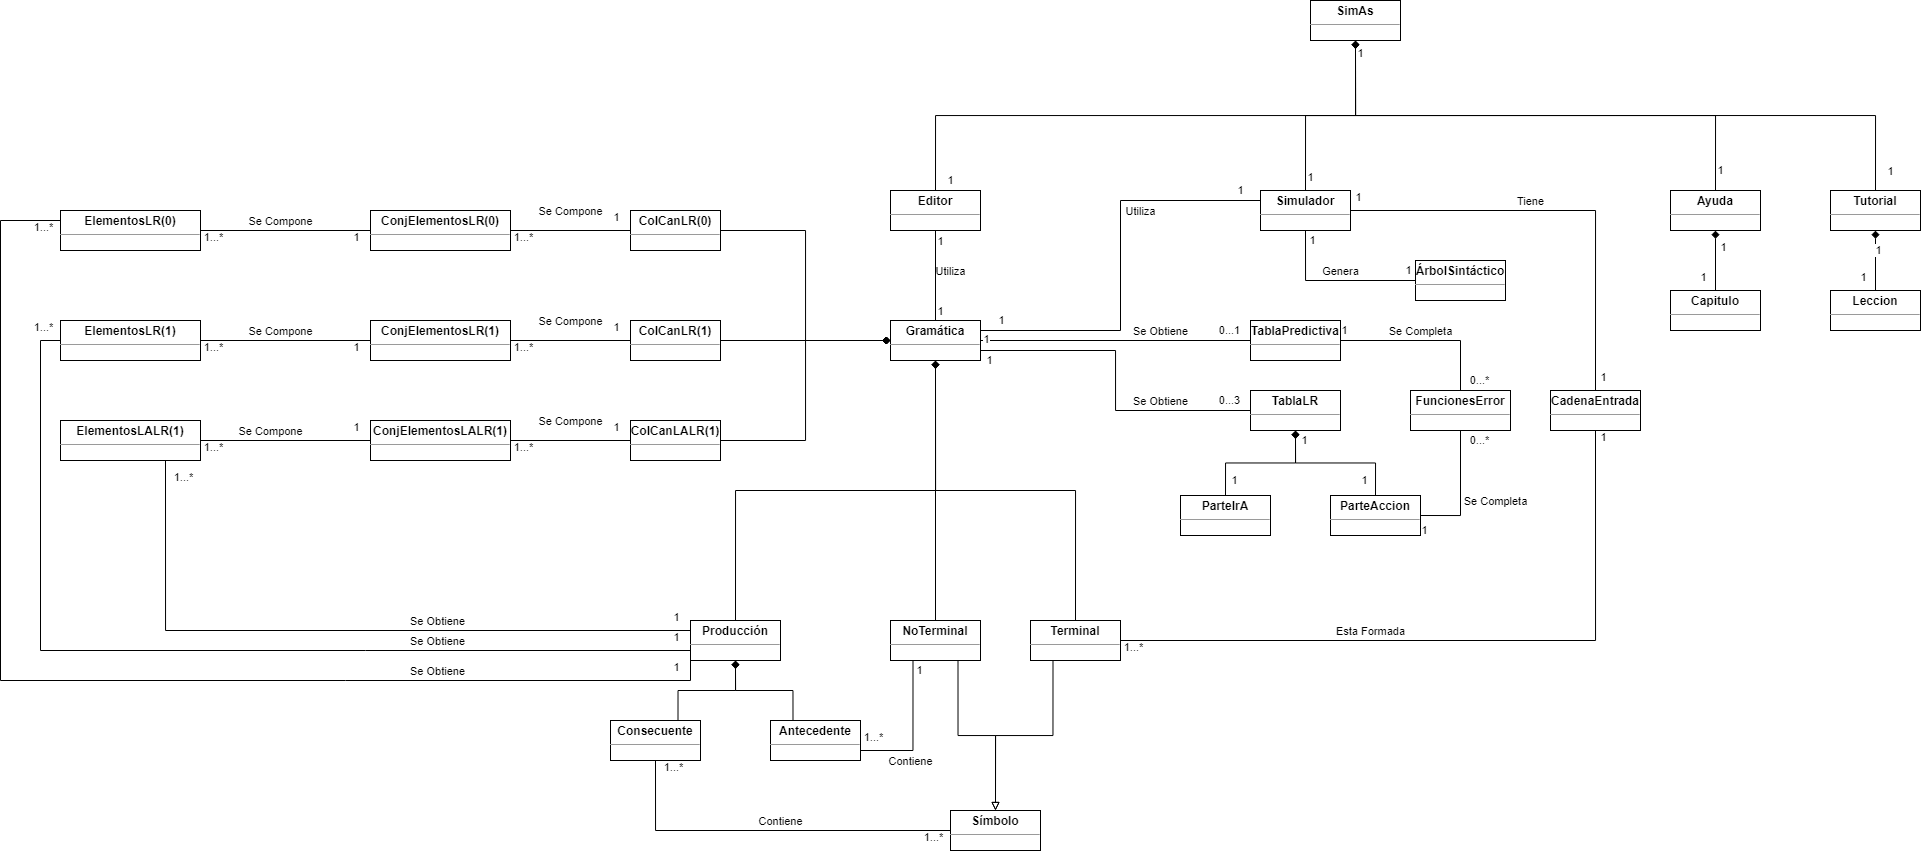
\includegraphics[width=0.9\textwidth]{figuras/Cap9/clases.png}
	\caption{Diagrama de clases de SimAS 3.0}
	\label{clases}
      \end{center}
  \end{figure}

El diagrama de clases muestra la arquitectura orientada a objetos de SimAS 3.0, destacando:

\begin{itemize}
    \item \textbf{Herencia}: La relación de herencia entre \textit{Simbolo} y sus subclases \textit{Terminal} y \textit{NoTerminal}.
    \item \textbf{Composición}: Las relaciones de composición entre \textit{Gramatica} y sus componentes (\textit{Produccion}, \textit{Terminal}, \textit{NoTerminal}, \textit{TablaPredictiva}).
    \item \textbf{Agregación}: Las relaciones de agregación entre \textit{Produccion} y sus partes (\textit{Antecedente}, \textit{Consecuente}).
    \item \textbf{Asociación}: Las relaciones de asociación entre las diferentes clases del modelo.
\end{itemize}

Esta arquitectura de clases proporciona una base sólida y extensible para el manejo de gramáticas de contexto libre en SimAS 3.0, siguiendo principios de diseño orientado a objetos y patrones de diseño como MVC (Model-View-Controller).